\documentclass[12pt]{article}
\bibliographystyle{unsrt}

\usepackage{a4wide}
\usepackage{amsmath}
\usepackage{amssymb}
\usepackage{booktabs}
\usepackage{graphicx}
\usepackage{url}

\usepackage{listings}
\usepackage{xcolor}

\definecolor{codegreen}{rgb}{0,0.6,0}
\definecolor{codegray}{rgb}{0.5,0.5,0.5}
\definecolor{codepurple}{rgb}{0.58,0,0.82}
\definecolor{backcolour}{rgb}{0.95,0.95,0.92}

\lstdefinestyle{mystyle}{
    backgroundcolor=\color{backcolour},   
    commentstyle=\color{codegreen},
    keywordstyle=\color{magenta},
    numberstyle=\tiny\color{codegray},
    stringstyle=\color{codepurple},
    basicstyle=\ttfamily\footnotesize,
    breakatwhitespace=false,         
    breaklines=true,                 
    captionpos=b,                    
    keepspaces=true,                 
    numbers=left,                    
    numbersep=5pt,                  
    showspaces=false,                
    showstringspaces=false,
    showtabs=false,                  
    tabsize=2
}

\lstset{style=mystyle}

\usepackage{color}
\definecolor{comment}{rgb}{0,0.3,0}
\definecolor{identifier}{rgb}{0.0,0,0.3}
\usepackage{listings}
\lstset{language=C++}
\lstset{
  columns=flexible,
  basicstyle=\tt\small,
  keywordstyle=,
  identifierstyle=\color{black},
  commentstyle=\tt\color{comment},
  mathescape=true,
  escapebegin=\color{comment},
  showstringspaces=false,
  keepspaces=true
}
\usepackage{hyperref}

\addtolength{\textwidth}{2cm}
\addtolength{\oddsidemargin}{-1cm}
\addtolength{\textheight}{2cm}
\addtolength{\topmargin}{-2cm}

\parskip 3pt
\newcommand{\etal}{\textit{et al}.}
\newcommand{\ie}{\textit{i}.\textit{e}.}
\newcommand{\eg}{\textit{e}.\textit{g}.}


\begin{document}
  
  \title{\sf MPLAPACK version 1.0.0 user manual}
  \author{NAKATA Maho$^1$\\
  \normalsize
  $^1$RIKEN Cluster for Pioneering Research, 2-1 Hirosawa, Wako-City, Saitama 351-0198, JAPAN}

\date{}

\maketitle

\begin{abstract}
The MPLAPACK (formerly MPACK) is a multiple-precision version of LAPACK \\
(\url{https://www.netlib.org/lapack/}).
MPLAPACK version 1.0.0 is based on LAPACK version 3.9.1 and translated from Fortran 90 to C++ using FABLE, a Fortran to C++ source-to-source conversion tool (\url{https://github.com/cctbx/cctbx\_project/tree/master/fable/}). 
MPLAPACK version 1.0.0 provides the real and complex version of MPBLAS, and the real version of MPLAPACK supports all LAPACK features: solvers for systems of simultaneous linear equations, least-squares solutions of linear systems of equations, eigenvalue problems, and singular value problems, and related matrix factorizations except for rectangular complete packed matrix form and mixed-precision routines. Besides, MPLAPACK supports a part of the complex routines of LAPACK, such as diagonalization of Hermite matrices, Cholesky factorization, and matrix inversion. The MPLAPACK defines an API for numerical linear algebra, similar to LAPACK. It is easy to port legacy C/C++ numerical codes using MPLAPACK. MPLAPACK supports binary64, binary128, FP80 (extended double), MPFR, GMP, and QD libraries (double-double and quad-double). Users can choose MPFR or GMP for arbitrary accurate calculations, double-double or quad-double for fast 32 or 64 decimal calculations. We can consider the binary64 version as the C++ version of LAPACK. MPLAPACK is available at GitHub (\url{https://github.com/nakatamaho/mplapack/}) under 2-clause BSD license.
\end{abstract}

\section{Introduction}

Numerical linear algebra aims to solve mathematical problems, such as simultaneous linear equations, eigenvalue problems, and least-squares methods, using arithmetic with finite-precision on a computer~\cite{GoluVanl96}. We can formulate many problems as numerical linear algebra in various fields, such as natural science, social science, and engineering. Therefore, its importance is magnificent. 

The standards for the numerical linear algebra package are BLAS~\cite{10.1145/567806.567807} and LAPACK~\cite{laug}. The BLAS library defines how computers should perform for vector, matrix-vector, and matrix-matrix operations in FORTRAN77. Almost all other vector and matrix arithmetic libraries are compatible with it or have very similar interfaces. Furthermore, LAPACK solves linear problems such as solving linear equations, singular value problems, eigenvalue problems, and least-square fitting problems using BLAS as a building block.

The main focus in numerical linear algebra has been on the speed and the size of solving the problem at approximately 8 or 16 decimal digits (binary32 or 64) using highly optimized BLAS and LAPACK~\cite{4610935,10.1145/1356052.1356053,6413635,8519659,cublas,tdb10}. Using higher precision numbers than binary64 is not common.

However, there are some problems in numerical linear algebra that require higher precision operations. In particular, when we solve ill-conditioned problems, large-scale simulations, and compute inversions of matrices, we usually need functions of higher precision numbers~\cite{BAILEY201210106,math3020337,high:ASNA2}.

Solving positive semidefinite programming (SDP) is yet another example that requires multi-precision computation. When we solve this problem using binary64 usually yields values up to eight decimal digits. The accumulation of numerical error occurs because the matrices' condition number at the optimal solution usually becomes infinite. As a result, Cholesky factorization fails near the optimal solution; the approximate solution diverges toward the optimal solution using the primal and dual interior point method~\cite{SDP}. Therefore, we require multiple precision calculations if we need more than eight decimal digits for optimal solutions. For this reason, we have developed SDPA-GMP~\cite{JCP2008,SDPA-GMP,SDPA}, the GNU MP version of semidefinite programming solver based on SDPA~\cite{SDPA}, which is one of the fastest SDP solvers.

MPLAPACK was developed as a drop-in replacement for BLAS and LAPACK in SDPA since SDPA performs Cholesky decomposition and solves symmetric eigenvalue problems via 50 BLAS and LAPACK routines~\cite{sdpa-gmpgithub}.

The features of MPLAPACK are:
\begin{itemize}
\item Provides Application Programming Interface (API) numerical algebra, similar to LAPACK and BLAS. Like BLAS and LAPACK, we can implement an optimized version of MPBLAS and MPLAPACK. In addition, we provide a simple OpenMP version of some MPBLAS routines as proof of concept.
\item Completely rewrote LAPACK and BLAS in C++ using FABLE and f2c.
\item C style programming. We do not introduce new matrix and vector classes. 
\item Supports seven floating-point formats by precision independent programming; binary64 (16 decimal digits), binary128 (32 decimal digits), FP80 (extended double; 19 decimal digits), double-double (32 decimal digits), quad-double (64 decimal digits), GMP, and MPFR (arbitrary precision, and the default is 153 decimal digits).
\item MPLAPACK 1.0.0 is based on LAPACK 3.9.1.
\item Version 1.0.0 supports all real and complex versions of BLAS and real version LAPACK functions; simultaneous linear equations, least-squares solutions of linear systems of equations, eigenvalue problems, and singular value problems and related matrix factorization except for mixed-precision version, and full packed matrix form version and complex version will be supported in version 2.0.
\item Reliability: We extended the original test programs to handle multiple-precision numbers, and most of the MPLAPCK routines have passed the test.
\item Runs on Linux/Windows/Mac.
\item Released at \url{https://github.com/nakatamaho/mplapack/} under 2-BSD clause license. 
\end{itemize}


The rest of the sections are organized as follows: Section~\ref{sec:supportedcpu} describes supported CPUs, OSes, and compilers. Section~\ref{sec:howtoinstall} describes how to install. Section~\ref{sec:floatingpointformat} describes the supported floating-point format. Section~\ref{sec:nameconventions} illustrates LAPACK and BLAS routine naming conventions and available MPBLAS and MPLAPACK routines; section~\ref{sec:howtouse} describes how to use MPBLAS and MPLAPACK. The examples are based on the assumption that users use Docker to avoid over-complicating the notation with differences in environments.
Section~\ref{sec:howtotest} describes how we tested MPBLAS and MPLAPACK.
Section~\ref{sec:howtoconvert} describes how we rewrote Fortran90 codes to C++ and extended them to multiple precision versions. Next, section ~\ref{sec:benchmarks} describes benchmarking MPBLAS routines, and section~\ref{sec:history} describes the history, Section~\ref{sec:relatedworks} describes related works. Finally, section~\ref{sec:futureplans} describes future plans for MPLAPACK. 

\section{Supported CPUs, OSes, and compilers}
\label{sec:supportedcpu}
Only 64 bit CPU is supported. Following OSes are supported:

\begin{itemize}
\item CentOS 7 (amd64, aarch64)
\item CentOS 8 (amd64, aarch64)
\item Ubuntu 20.04 (amd64, aarch64)
\item Ubuntu 18.04 (amd64)
\item Windows 10 (amd64)
\item MacOS (Intel)
\end{itemize}

We support the following compilers:
\begin{itemize}
\item GCC (GNU Compiler Collection) 9 and 10
\item Intel OneAPI.
\end{itemize}
Note that we use GCC by MacPorts on macOS, which is NOT the default compiler. We use the mingw64 and Wine64 environments on Linux to build and test the Windows version. On different configurations, MPLAPACK may build and work without problems. We welcome patches from the community.

\section{Installation}
\label{sec:howtoinstall}
\subsection{Using Docker (recommended for Linux environment)}
The easiest way to install MPLAPACK is to build inside Docker~\cite{merkel2014docker} and use it inside Docker. 
For example, the following command will build inside docker on Ubuntu amd64 (also known as x86\_64) or aarch64 (also known as arm64); the following command will build inside docker.

\begin{verbatim}
$ git clone https://github.com/nakatamaho/mplapack/
$ cd mplapack
$ /usr/bin/time docker build -t mplapack:ubuntu2004 -f Dockerfile_ubuntu20.04 . \
   2>&1 | tee log.ubuntu2004
\end{verbatim}

In Table~\ref{dockerfiles}, we list corresponding Dockerfiles for CPU and OS. 

When the build is finished, all the files will be installed under $\tt /home/docker/MPLAPACK$.

One can also install MPLAPACK in the desired directry. First, make a tar archive of installed directory,
\begin{verbatim}
$ docker run -it mplapack:ubuntu2004
$ cd /home/docker/MPLAPACK
$ tar cvfz ../mplapack.tar.gz .
$ cd .. ; scp mplapack.tar.gz YourhostIP:
$ exit
\end{verbatim}
Then, on the host OS, copy like following:
\begin{verbatim}
$ sudo tar xvfz mplapack.tar.gz -C /usr/local/mplapack
\end{verbatim}
In Table~\ref{dockerfiles}, we list Dockerfiles and corresponding CPU, OS, and compiler.

\begin{table}
\caption{The name of the Dockerfile and the corresponding OS and CPU}\label{dockerfiles}
\begin{center}
\begin{tabular}{l|c|c|c}
Docker filename                      & CPU          & OS            & Compiler \\ \hline
\tt Dockerfile\_CentOS7              & amd64        & CentOS 7       & GCC \\
\tt Dockerfile\_CentOS7\_AArch64     & aarch64 only & CentOS 7       & GCC\\
\tt Dockerfile\_CentOS8              & all CPUs     & CentOS 8  & GCC \\
\tt Dockerfile\_ubuntu18.04          & amd64 only   & Ubuntu 18.04 & GCC  \\
\tt Dockerfile\_ubuntu20.04          & all CPUs     & Ubuntu 20.04  & GCC\\
\tt Dockerfile\_ubuntu20.04\_intel   & amd64 only   & Ubuntu 20.04  & Intel oneAPI \\
\tt Dockerfile\_ubuntu20.04\_mingw64 & amd64 only   & Windows10     & GCC \\ \hline
\end{tabular}
\end{center}
\end{table}

\subsection{Compiling from the source}
We list prerequisites for compiling from the source in Table~\ref{prerequisites}; users can satisfy these prerequisites using MacPorts on macOS. Homebrew may be used as an alternative to satisfy these prerequisites.

\begin{verbatim}
$ sudo port install gcc9 coreutils git ccache
$ git clone https://github.com/nakatamaho/mplapack.git --depth 1
$ cd mplapack
$ pushd mplapack/debug ; bash gen.Makefile.am.sh ; popd
$ autoreconf --force --install ; aclocal ; autoconf ; automake
$ autoreconf --force --install
$ CXX="g++-mp-9" ; export CXX
$ CC="gcc-mp-9" ; export CC
$ FC="gfortran-mp-9"; export FC
$ F77="gfortran-mp-9"; export F77
$ ./configure --prefix=/Users/maho/MPLAPACK --enable-gmp=yes --enable-mpfr=yes \
--enable-_Float128=yes --enable-qd=yes --enable-dd=yes --enable-double=yes \
--enable-_Float64x=yes --enable-test=yes
...
$ make -j6
...
$ make install
\end{verbatim}

\begin{table}
\caption{Prerequisites for compiling from source}
\begin{center}\label{prerequisites}
\begin{tabular}{lc}
Package & Version \\ \hline
gcc & 9 or later \\
gmake & 4.3 or later \\
git & 2.33.0 or later\\
gsed & 4.8 or later \\
autotools & 2.71 \\
automake & 1.16 \\ 
GNU sed & 4.1 or later \\ 
\hline
\end{tabular}
\end{center}
\end{table}

\section{Supported Floating point formats}
\label{sec:floatingpointformat} 
We support binary64, FP80 (extended double), binary128, double-double, quad-double (QD library), GMP, and MPFR in MPLAPACK. 

Binary64~\cite{4610935} is the so-called double precision: the number of significant digits in decimal is about 16, and CPUs perform arithmetic processing in hardware. As a result, the CPU can perform binary64 operations very fast.

FP80 is an extended double precision. IEEE 754-1985 species the minimum requirements for an extended double format~\cite{30711}, and 80-bit format meets the minimum requirement. FP80 has approximately 19 digits accuracy, respectively and FP80 has a much wider exponent than binary64. Recently, ISO defined C real floating type~\cite{18661-3} for FP80 as {\tt \_Float64x} but not yet a standard of C++. Moreover, GCC has already defined type for FP80 as {\tt \_\_float80}. In any case, we always use {\tt \_Float64x} MPLAPACK programs to keep the consistency among different environments. When building the MPLAPACK library, the configure script investigates whether {\tt \_Float64x} is available or not. If not, we typedef the appropriate type as ${\tt \_Float64x}$. Only Intel and AMD CPUs support FP80 format. These CPUs implement FP80 as hardware. However, they do not support SIMD-type acceleration like SSE nor AVX; thus, FP80 arithmetic is much slower than binary64.

Binary128, and sometimes called quadruple precision, is defined in IEEE754-2008 \cite{4610935} and this format has approximately 33 decimal significant digits. Usually binary128 arithmetic is done by software, therefore, operations are very slow. As far as we know, only IBM z processors have been the only commercial platform supporting quadruple-precision \cite{IBMz13}. Some processors like aarch64, Sparc, RISCV64, MIPS64 define instructions for quadruple-precision arithmetic. These processors emulate binary128 instructions by software. ISO defined C real floating types~\cite{18661-3} as {\tt \_Float128} but not yet a standard of C++. GCC has already been providing a type for binary128 as {\tt \_\_float128}. We always use {\tt \_Float128} as a type for binary128 numbers in MPLAPACK. This type may be the same as {\tt long double} or {\tt \_\_float128} depends on the environment, we typedef appropriate type to {\tt \_Float128}.
 
We use the QD library \cite{hida2000} to support double-double and quad-double precision. The double-double casts two binary64 numbers as a one number and has approximately 32 decimal significant digits, and the quad-double casts four binary64 numbers as a one number and has approximately 64 decimal significant digits. Using Kunth and Dekker's algorithm \cite{Knuth1997,Dekker1971}, which can evaluate the addition and multiplication of two binary64 numbers exactly. Then, we can define the addition and multiplication of double-double numbers. Pros for using these format is speed. Since all arithmetic can be done by binary64 and accelerated by hardware, calculation speed is are approximately ten times faster than software implemented binary128. Cons of using these formats are programs written for expecting IEEE754 feature might not work with these precisions. Note that OSes and compilers for IBM Power CPU and Power Macs, ``long double" has been equivalent to the double-double.

GMP~\cite{Granlund12} is a C library for arbitrary precision arithmetic, operating on signed integers, rational numbers, and floating-point numbers. We can perform calculations to any accuracy, as long as the machine's resources allow. We support complex numbers by preparing ${\tt mpc\_class}$. 

MPFR~\cite{10.1145/1236463.1236468} is a C library for multiple-precision floating-point computations with correct rounding based on GMP. We support complex numbers using MPC, which is a library for multiple-precision complex arithmetic with correct rounding~\cite{MPC} via ${\tt mpcomplex}$ class. Both libraries provide almost the same functionalities, but MPFR and MPC further support trigonometric functions necessary for cosine-sine decomposition, elementary and special functions. Therefore, we will drop GMP support in the future.

{\tt long double} is no longer supported in MPLAPACK since v1.0.0 since the situation regarding {\tt long double} is very different and confusing in different environments. E.g., on Intel CPUs, {\tt long double} may be equivalent to {\tt \_Float64x}; however, it also depends on OSes. On Windows, {\tt long double} is equivalent to {\tt double}. Similar confusion happens in the AArch64 environment. ARM defines {\tt long double} should be binary64, but on the OS side, Apple overwrites {\tt long double} should be double. On IBM PowerPC or Power Macs, {\tt long double} have been double-double.

\section{LAPACK and BLAS Routine Naming Conventions and available routines}
\label{sec:nameconventions}
BLAS and LAPACK prefix routine names with ``s" and ``d" for (real) single and double precision real numbers and ``c" and ``z" for single and double precision complex numbers. FORTRAN77 and Fortran90 are not case-sensitive in function and subroutine names, while C++ is case-sensitive in function names.

The prefix for real and complex routine names in MPLAPACK is an uppercase ``R" for real numbers and ``C" for complex numbers. All other letters in the routines are lowercase.
Also, while we do not distinguish function names by floating-point class (e.g. {\tt mpf\_class, \_Float128}), we use the same function name for different floating-point classes to take advantage of function overloading (e.g., no matter which floating-point class is adopted, program calls {\tt Raxpy} appropriately). The floating-point class is added after the routine name for routines that take no arguments or only integers. Otherwise, we add the prefix ``M" or insert ``M" after ``i."

For example, \begin{itemize}
    \item {\tt daxpy, zaxpy $\rightarrow$ Raxpy, Caxpy}
    \item {\tt dgemm, zgemm $\rightarrow$ Rgemm, Cgemm}
    \item {\tt dsterf, dsyev $\rightarrow$ Rsterf, Rsyev}
    \item {\tt dzabs1, dzasum $\rightarrow$ RCabs1, RCasum}
    \item {\tt lsame $\rightarrow$ Mlsame\_mpfr,  Mlsame\_gmp, Mlsame\_\_Float128} $\cdots$ etc.
    \item {\tt dlamch $\rightarrow$ Rlamch\_mpfr,  Rlamch\_gmp, Rlamch\_\_Float128} $\cdots$ etc.
    \item {\tt ilaenv $\rightarrow$ iMlaenv\_mpfr,  iMlaenv\_gmp, iMlaenv\_\_Float128} $\cdots$ etc.
\end{itemize}

In table~\ref{mpblasroutines}, we show all supported MPBLAS routines.
The prototype definitions of these routines can be found in the following headers.
\begin{itemize} 
\item {\tt /home/docker/MPLAPACK/include/mplapack/mpblas\_\_Float128.h}
\item {\tt /home/docker/MPLAPACK/include/mplapack/mpblas\_\_Float64x.h}
\item {\tt /home/docker/MPLAPACK/include/mplapack/mpblas\_dd.h}
\item {\tt /home/docker/MPLAPACK/include/mplapack/mpblas\_double.h}
\item {\tt /home/docker/MPLAPACK/include/mplapack/mpblas\_gmp.h}
\item {\tt /home/docker/MPLAPACK/include/mplapack/mpblas\_mpfr.h}
\item {\tt /home/docker/MPLAPACK/include/mplapack/mpblas\_qd.h}
\end{itemize}
A simple OpenMP version of MPBLAS is available.
In table~\ref{mpblasroutinesopt}, we show all OpenMP accelerated MPBLAS routines. \\

In table~\ref{mplapackdriver}, we show all supported MPLAPACK driver routines.
In table~\ref{mplapackcomp}, we show all supported MPLAPACK Real computational routines.
In table~\ref{mplapackcomp_complex}, we show all supported MPLAPACK complex computational routines.

We do not list here, but there are many MPLPACK auxiliary routines as well.

We usually use MPLAPACK driver routines and MPBLAS routines directly. MPLAPACK computational routines and auxiliary routines
may be implicitly used by the driver routines. 

The prototype definitions of the MLAPACK routines can be found in the following headers.
\begin{itemize}
\item {\tt /home/docker/MPLAPACK/include/mplapack/mplapack\_\_Float128.h}
\item {\tt /home/docker/MPLAPACK/include/mplapack/mplapack\_\_Float64x.h}
\item {\tt /home/docker/MPLAPACK/include/mplapack/mplapack\_dd.h}
\item {\tt /home/docker/MPLAPACK/include/mplapack/mplapack\_double.h}
\item {\tt /home/docker/MPLAPACK/include/mplapack/mplapack\_gmp.h}
\item {\tt /home/docker/MPLAPACK/include/mplapack/mplapack\_mpfr.h}
\item {\tt /home/docker/MPLAPACK/include/mplapack/mplapack\_qd.h}
\end{itemize}

\begin{table}
\caption{Available MPBLAS routines}\label{mpblasroutines}
\begin{center}
{\tt
\begin{tabular}{cccccccccc} \hline
Crotg & Cscal & Rrotg & Rrot & Rrotm & CRrot & Cswap & Rswap & CRscal & Rscal \\
Ccopy & Rcopy & Caxpy & Raxpy & Rdot & Cdotc  & Cdotu & RCnrm2 & Rnrm2 & Rasum \\
iCasum & iRamax & RCabs1& Mlsame & Mxerbla \\ \hline
Cgemv & Rgemv & Cgbmv & Rgbmv & Chemv & Chbmv & Chpmv & Rsymv & Rsbmv & Ctrmv \\
Cgemv & Rgemv & Cgbmv & Rgemv & Chemv & Chbmv & Chpmv & Rsymv & Rsbmv & Rspmv \\
Ctrmv & Rtrmv & Ctbmv & Ctpmv & Rtpmv & Ctrsv & Rtrsv & Ctbsv & Rtbsv & Ctpsv \\
Rger  & Cgeru & Cgerc & Cher  & Chpr & Cher2  & Chpr2  & Rsyr  & Rspr & Rsyr2 \\
Rspr2 \\ \hline
Cgemm & Rgemm & Csymm & Rsymm & Chemm & Csyrk  & Rsyrk & Cherk & Csyr2k& Rsyr2k \\
Cher2k& Ctrmm & Rtrmm & Ctrsm & Rtrsm\\\hline
\end{tabular}
}
\end{center}
\end{table}

\begin{table}
\caption{Available OpenMP version of MPBLAS routines}\label{mpblasroutinesopt}
\begin{center}
{\tt
\begin{tabular}{cccccccccc} \hline
Raxpy & Rcopy & Rdot & Rgemm \\ \hline
\end{tabular}
}
\end{center}
\end{table}


\begin{table}
\caption{Available MPLAPACK Driver routines (1.0.0)}\label{mplapackdriver}
\begin{center}
{\tt 
\begin{tabular}{cccccccccc} \hline
Rgesv  & Rgesvx & Rgbsv  & Rgbsvx & Rgtsv & Rgtsvx & Rposv  & Rposvx & Rppsv  & Rppsvx \\
Rpbsv  & Rpvsvx & Rptsv  & Rptsvx & Rsysv & Rsysvx & Rpspv  & Rspsvx & Rgels  & Rgelsy \\
Rgelss & Rgelsd & Rgglse & Rggglm & Rsyev & Rsyevd & Rsvevd & Rsyevr & Rsepev & Rspevd \\
Rspevx & Rsbev & Rsbevd & Rsbevx & Rstev & Rstevd  & Rstevx & Rstevr & Rgees & Rgeesx \\
Rgeev & Rgeevx & Rgesvd & Rgesdd & Rsygv & Rsygvd & Rsygvx & Rspgv & Rspgdv & Rspgvx \\
Rsbgv & Rsbgv & Rsbgvx & Rgges  & Rggesx & Rggev & Rggevx & Rggsvd \\ \hline
\end{tabular}
}
\end{center}
\end{table}

\begin{table}
\caption{Available MPLAPACK Computational Real routines (1.0.0)}\label{mplapackcomp}
\begin{center}
{\tt
\begin{tabular}{cccccccccccc} \hline
Rgetrf & Rgetrs & Rgecon & Rgerfs & Rgetri & Rgeequ & Rgbtrf & Rgbtrs & Rgbcon & Rgbrfs \\
Rgbequ & Rgttrf & Rgttrs & Rgtcon & Rgtrfs & Rpotrf & Rpotrs & Rpocon & Rporfs & Rpotri \\
Rpoequ & Rpptrf & Rpptrs & Rppcon & Rpprfs & Rpptri & Rppequ & Rpbtrf & Rpbtrs & Rpbcon \\
Rpbrfs & Rpbequ & Rpttrf & Rpttrs & Rptcon & Rptrfs & Rsytrf & Rsytrs & Rsycon & Rsyrfs \\
Rsytri & Rsptrf & Rsptrs & Rspcon & Rsprfs & Rsptri & Rtrtrs & Rtrcon & Rtrrfs & Rtrtri \\
Rtptrs & Rtpcon & Rtprfs & Rtptri & Rtbtrs & Rtbcon & Rtbrfs \\ \hline
Rgeqp3 & Rgeqrf & Rorgqr & Rormqr & Rgelqf & Rorglq & Rormlq & Rgeqlf & Rorgql & Rormql \\
Rgerqf & Rorgrq & Rormrq & Rtzrzf & Rormrz \\ \hline
Rsytrd & Rsptrd & Rsbtrd & Rorgtr & Rormtr & Ropgtr & Ropmtr & Rsteqr & Rsterf & Rstedc \\
Rstegr & Rstebz & Rstein & Rpteqr \\ \hline
Rgehrd & Rgebal & Rgebak & Rorghr & Rormhr & Rhseqr & Rhsein & Rtrevc & Rtrexc & Rtrsyl \\
Rtrsna & Rtrsen \\ \hline
Rgebrd & Rgbbrd & Rorgbr & Rormbr & Rbdsqr & Rbdsdc \\ \hline
Rsygst & Rspgst & Rpbstf & Rsbgst \\ \hline
Rgghrd & Rggbal & Rggbak & Rhgeqz & Rtgevc & Rtgexc & Rtgsyl & Rtgsna & Rtgsen \\ \hline
Rggsvp & Rtgsja \\
\hline
\end{tabular}
}
\end{center}
\end{table}

\begin{table}
\caption{Available MPLAPACK Computational Complex routines (1.0.0)}\label{mplapackcomp_complex}
\begin{center}
{\tt
\begin{tabular}{cccccccccccc} \hline
Cgelq2 & Cgeqr2 & Cgeqrf & Cgesv  & Cgetf2 & Cgetrf & Cgetri & Cgetrs & Cheev  & Chetd2 \\
Chetrd & Clacgv & Clacrm & Clacrt & Cladiv & Claesy & Claev2 & Clahef & Clanhe & Clanht \\
Clansy & Clarfb & Clarfg & Clarf  & Clarft & Clartg & Clascl & Claset & Clasr & Classq \\
Claswp & Clasyf & Clatrd & Cpotf2 & Crot   & Cspmv  &  Cspr & Csteqr  & Csymv & Csyr \\
Ctrti2 & Ctrtri & Ctrtrs & Cung2l & Cung2r & Cungql & Cungqr & Cungtr & Cunmqr \\ \hline
\end{tabular}
}
\end{center}
\end{table}

%%wget https://www.netlib.org/lapack/lug/node59.html^C
%% maho@DESKTOP-MP6PMVB:~$ grep TD node59.html  | sed 's/<TD ALIGN="LEFT">//g' | grep ^D | sed 's/</ /g'  | awk '{print $1}' |  tr "[A-Z]" "[a-z]" | awk '{ print toupper(substr($0, 1, 1)) substr($0, 2, length($0) - 1) }'  | sed 's/D/R/g'  | awk '{print $1 " &" }' | tr "\n" " ";echo
\section{How to use MPBLAS and MPLPACK}
\label{sec:howtouse}
\subsection{Types}
We use seven kinds of floating-point formats. Multiple precision types are listed in the table~\ref{mplapackformats}.
For GMP, we use built-in {\tt mpf\_class} for real type. For complex type, we developed {\tt mpc\_class}.
For MPFR, we use a modified version of mpfrc++ (the final LGPL version) to treat like double or float type. For complex type,
we developed {\tt mpcomplex.h} using MPFR and MPC.
For double-double and quad-double, we use {\tt dd\_real} and {\tt qd\_real}, respectively. For complex type, we developed {\tt dd\_complex} and {\tt qd\_complex}, respectively.

For extended double we use {\tt \_Float64x} for all Intel and AMD environment. For binary128, we use {\_Float128} for
all OSes and CPUs. For complex types for {\tt double}, {\tt \_Float64x} and {\tt \_Float128}, we use standard complex implementation of C++. Using {\tt \_\_float80}, {\tt \_\_float128}, or {\tt long double} is strongly discouraged as they are not tested and not portable.

\begin{table}
\caption{The floating-point formats used in MPLAPACK, their type names, and accuracy in decimal digits.}\label{mplapackformats}
\begin{center}
\begin{tabular}{c|c|c} \hline
Library or format & type name & accuracy in decimal digits \\ \hline
GMP             & {\tt mpf\_class, mpc\_class}       & 154 (default) and arbitrary\\
MPFR            & {\tt mpreal, mpcomplex}            & 154 (default) and arbitrary \\
double-double   & {\tt dd\_real, dd\_complex}        & 32\\
quad-double     & {\tt qd\_real, qd\_complex}        & 64 \\
binary64        & {\tt double, std::complex<double>} & 16 \\
extended double & {\tt \_Float64x, std::complex<\_Float64x>} & 19  \\
binary128       & {\tt \_Float128, std::complex<\_Float128>} & 33 \\ 
integer         & mplapackint & (32bit on Win, 64bit on Linux and macOS) \\ \hline
\end{tabular}
\end{center}
\end{table}
Also, we define {\tt mplapackint} as a 64 bit signed integer to MPLAPACK that can access all the memory spaces regardless
of which data type models the environment employs (LLP64 or LP64). On Windows, {\tt mplapackint} is still a 32 bit signed integer.


\subsection{MPBLAS}
The API of MPBLAS is very similar to the original BLAS and CBLAS. However, we always use a one-dimensional array as a column-major type matrix in MPBLAS, and unlike CBLAS, we cannot specify row- or column-major order. 

Following is the prototype definition of the multiple-precision version of matrix-matrix multiplication ({\tt Rgemm}) by MPFR.
\begin{verbatim}
void Rgemm(const char *transa, const char *transb, mplapackint const m, 
mplapackint const n, mplapackint const k, mpreal const alpha, mpreal *a, 
mplapackint const lda, mpreal *b, mplapackint const ldb, mpreal const beta, 
mpreal*c, mplapackint const ldc);
\end{verbatim}
and the following is the definition part of the original DGEMM 
\begin{verbatim}
SUBROUTINE DGEMM(TRANSA,TRANSB,M,N,K,ALPHA,A,LDA,B,LDB,BETA,C,LDC)
*     .. Scalar Arguments ..
      DOUBLE PRECISION ALPHA,BETA
      INTEGER K,LDA,LDB,LDC,M,N
      CHARACTER TRANSA,TRANSB
*     ..
*     .. Array Arguments ..
      DOUBLE PRECISION A(LDA,*),B(LDB,*),C(LDC,*)
\end{verbatim}
There is correspondence between variables in the C++ prototype of Rgemm and variables in the header of {\tt DGEMM}.
\begin{itemize}
    \item {\tt CHARACTER} $\rightarrow$ {\tt const char *}
    \item {\tt INTEGER} $\rightarrow$ {\tt mplapackint}
    \item {\tt DOUBLE PRECISION A(LDA, *)} $\rightarrow$ {\tt mpreal *a}
\end{itemize}
We can see such correspondences for other MPBLAS and MPLAPACK routines.
Let us see how we can multiply matrices using MPFR. 
The list is the following.
\begin{lstlisting}
#include <mpblas_mpfr.h>

//Matlab/Octave format
void printmat(int N, int M, mpreal * A, int LDA)
{
    mpreal mtmp;
    printf("[ ");
    for (int i = 0; i < N; i++) {
        printf("[ ");
        for (int j = 0; j < M; j++) {
            mtmp = A[i + j * LDA];
            mpfr_printf("%5.2Re", mpfr_ptr(mtmp));
            if (j < M - 1)
                printf(", ");
        }
        if (i < N - 1)
            printf("]; ");
        else
            printf("] ");
    }
    printf("]");
}

int main()
{
    mplapackint n = 3;
//initialization of MPFR
    int default_prec = 256;
    mpfr_set_default_prec(default_prec);

    mpreal *A = new mpreal[n * n];
    mpreal *B = new mpreal[n * n];
    mpreal *C = new mpreal[n * n];
    mpreal alpha, beta;

//setting A matrix
    A[0 + 0 * n] = 1;    A[0 + 1 * n] = 8;    A[0 + 2 * n] = 3;
    A[1 + 0 * n] = 0;    A[1 + 1 * n] = 10;   A[1 + 2 * n] = 8;
    A[2 + 0 * n] = 9;    A[2 + 1 * n] = -5;   A[2 + 2 * n] = -1;

    B[0 + 0 * n] = 9;    B[0 + 1 * n] = 8;    B[0 + 2 * n] = 3;
    B[1 + 0 * n] = 3;    B[1 + 1 * n] = -11;  B[1 + 2 * n] = 0;
    B[2 + 0 * n] = -8;   B[2 + 1 * n] = 6;    B[2 + 2 * n] = 1;

    C[0 + 0 * n] = 3;    C[0 + 1 * n] = 3;    C[0 + 2 * n] = 0;
    C[1 + 0 * n] = 8;    C[1 + 1 * n] = 4;    C[1 + 2 * n] = 8;
    C[2 + 0 * n] = 6;    C[2 + 1 * n] = 1;    C[2 + 2 * n] = -2;

    printf("# Rgemm demo...\n");

    printf("A ="); printmat(n, n, A, n); printf("\n");
    printf("B ="); printmat(n, n, B, n); printf("\n");
    printf("C ="); printmat(n, n, C, n); printf("\n");
    alpha = 3.0;
    beta = -2.0;
    Rgemm("n", "n", n, n, n, alpha, A, n, B, n, beta, C, n);

    mpfr_printf("alpha = %5.3Re\n", mpfr_ptr(alpha));
    mpfr_printf("beta  = %5.3Re\n", mpfr_ptr(beta));
    printf("ans ="); printmat(n, n, C, n); printf("\n");
    printf("#please check by Matlab or Octave following and ans above\n");
    printf("alpha * A * B + beta * C =\n");
    delete[]C;
    delete[]B;
    delete[]A;
}
\end{lstlisting}
First, we must include {\tt mpblas\_mpfr.h} to use MPFR. {\tt printmat} function prints matrix in Matlab format (lines 4 to 22). 
We set 256 bit in fraction for mpfrc++ in lines 28 to 29; MPFR Real accuracy setted to  77 decimal digits ($77.06 = \log_{10} 2^{256}$).
We allocate the matrix as a one-dimensional array (lines 31 to 33). Then we set the matrix $A$, $B$, and $C$. We always input matrix by row-major format to an array (lines36 to 47). Matrix-matrix multiplication {\tt Rgemm} is called in line 58. 
One can input the list and save as {\tt Rgemm\_mpfr.cpp} or you can find {\tt /home/docker/mplapack/examples/mpblas/} directory.
Then, one can compile by one own like following in Docker environment as follows:
\begin{verbatim}
$ g++ -O2 -I/home/docker/MPLAPACK/include -I/home/docker/MPLAPACK/include/mplapack \
Rgemm_mpfr.cpp -L/home/docker/MPLAPACK/lib -lmpblas_mpfr -lgmp -lmpfr -lmpc
\end{verbatim}
Then, you can run as follows:
{\fontsize{9.5pt}{0.4cm}\selectfont
\begin{verbatim}
$ LD_LIBRARY_PATH=/home/docker/MPLAPACK/lib ./a.out
# Rgemm demo...
A =[ [ 1.00e+00, 8.00e+00, 3.00e+00]; [ 0.00e+00, 1.00e+01, 8.00e+00]; [ 9.00e+00, -5.00e+00, -1.00e+00] ]
B =[ [ 9.00e+00, 8.00e+00, 3.00e+00]; [ 3.00e+00, -1.10e+01, 0.00e+00]; [ -8.00e+00, 6.00e+00, 1.00e+00] ]
C =[ [ 3.00e+00, 3.00e+00, 0.00e+00]; [ 8.00e+00, 4.00e+00, 8.00e+00]; [ 6.00e+00, 1.00e+00, -2.00e+00] ]
alpha = 3.000e+00
beta  = -2.000e+00
ans =[ [ 2.10e+01, -1.92e+02, 1.80e+01]; [ -1.18e+02, -1.94e+02, 8.00e+00]; [ 2.10e+02, 3.61e+02, 8.20e+01] ]
#please check by Matlab or Octave following and ans above
alpha * A * B + beta * C
\end{verbatim}
}
One can check the result by comparing the result of the octave.
{\footnotesize
\begin{verbatim}
$ LD_LIBRARY_PATH=/home/docker/MPLAPACK/lib ./a.out | octave
octave: X11 DISPLAY environment variable not set
octave: disabling GUI features
A =

    1    8    3
    0   10    8
    9   -5   -1

B =

    9    8    3
    3  -11    0
   -8    6    1

C =

   3   3   0
   8   4   8
   6   1  -2

alpha =  3
beta = -2
ans =

    21  -192    18
  -118  -194     8
   210   361    82

ans =

    21  -192    18
  -118  -194     8
   210   361    82
\end{verbatim}
}
In this case, we see the result below two ``{\tt ans =}'' are the same. The {\tt Rgemm} result is correct up to 16 decimal digits.

Let us see how we can multiply matrices using {\tt \_Float128} (binary128). The list is the following.
\begin{lstlisting}
#include <mpblas__Float128.h>
#include <stdio.h>
#define BUFLEN 1024

void printnum(_Float128 rtmp)
{
    int width = 42;
    char buf[BUFLEN];
#if defined ___MPLAPACK_WANT_LIBQUADMATH___
    int n = quadmath_snprintf (buf, sizeof buf, "%+-#*.35Qe", width, rtmp);
#elif defined ___MPLAPACK_LONGDOUBLE_IS_BINARY128___
    snprintf (buf, sizeof buf, "%.35Le", rtmp);
#else
    strfromf128(buf, sizeof(buf), "%.35e", rtmp);
#endif
    printf ("%s", buf);
    return;
}

//Matlab/Octave format
void printmat(int N, int M, _Float128 * A, int LDA)
{
    _Float128 mtmp;

    printf("[ ");
    for (int i = 0; i < N; i++) {
        printf("[ ");
        for (int j = 0; j < M; j++) {
            mtmp = A[i + j * LDA];
            printnum(mtmp);
            if (j < M - 1)
                printf(", ");
        }
        if (i < N - 1)
            printf("]; ");
        else
            printf("] ");
    }
    printf("]");
}

int main()
{
    mplapackint n = 3;

    _Float128 *A = new _Float128[n * n];
    _Float128 *B = new _Float128[n * n];
    _Float128 *C = new _Float128[n * n];
    _Float128 alpha, beta;

//setting A matrix
    A[0 + 0 * n] = 1;    A[0 + 1 * n] = 8;    A[0 + 2 * n] = 3;
    A[1 + 0 * n] = 2.5;  A[1 + 1 * n] = 10;   A[1 + 2 * n] = 8;
    A[2 + 0 * n] = 9;    A[2 + 1 * n] = -5;   A[2 + 2 * n] = -1;

    B[0 + 0 * n] = 9;    B[0 + 1 * n] = 8;    B[0 + 2 * n] = 3;
    B[1 + 0 * n] = 3;    B[1 + 1 * n] = -11;  B[1 + 2 * n] = 4.8;
    B[2 + 0 * n] = -8;   B[2 + 1 * n] = 6;    B[2 + 2 * n] = 1;

    C[0 + 0 * n] = 3;    C[0 + 1 * n] = 3;    C[0 + 2 * n] = 1.2;
    C[1 + 0 * n] = 8;    C[1 + 1 * n] = 4;    C[1 + 2 * n] = 8;
    C[2 + 0 * n] = 6;    C[2 + 1 * n] = 1;    C[2 + 2 * n] = -2;

    printf("# Rgemm demo...\n");

    printf("A ="); printmat(n, n, A, n); printf("\n");
    printf("B ="); printmat(n, n, B, n); printf("\n");
    printf("C ="); printmat(n, n, C, n); printf("\n");
    alpha = 3.0;
    beta = -2.0;
    Rgemm("n", "n", n, n, n, alpha, A, n, B, n, beta, C, n);

    printf("alpha = "); printnum(alpha); printf("\n");
    printf("beta  = "); printnum(beta);  printf("\n");
    printf("ans ="); printmat(n, n, C, n); printf("\n");
    printf("#please check by Matlab or Octave following and ans above\n");
    printf("alpha * A * B + beta * C \n");
    delete[]C;
    delete[]B;
    delete[]A;
}
\end{lstlisting}
We do not show the output since the output is almost the same as the MPFR version.

The {\tt \_Float128} version of progarm list is almost similar to the MPFR version, too. However, {\tt printnum} part is bit complicated. Because there are at least three kinds of binary128 support depend on CPUs and OSes: (i) GCC only supports {\tt \_\_float128} using {\tt libquadmath} (Windows, macOS), (ii) GCC supports {\tt \_Float128} directly and there are libc support as well (Linux amd64), (iii) {\tt long double} is already binary128 and no special support is necessary (AArch64). For (i), we internally define {\tt \_\_\_MPLAPACK\_WANT\_LIBQUADMATH\_\_\_}, for (ii) we define {\tt \_\_\_MPLAPACK\_\_FLOAT128\_ONLY\_\_\_}, and for (iii),
we define {\tt \_\_\_MPLAPACK\_LONGDOUBLE\_IS\_BINARY128\_\_\_}. Users can use these internal defines to write a portable program.

As a summary, we show how we compile and run binary64, FP80, binary128, double-double, quad-double, GMP and MPFR versions of {\tt Rgemm} demo programs in {\tt /home/docker/mplapack/examples/mpblas} as follows:
\begin{itemize}
    \item binary64 (double) version
\begin{verbatim}
$ g++ -O2 -I/home/docker/MPLAPACK/include -I/home/docker/MPLAPACK/include/mplapack \
Rgemm_double.cpp -L/home/docker/MPLAPACK/lib -lmpblas_double
$ LD_LIBRARY_PATH=/home/docker/MPLAPACK/lib ./a.out
\end{verbatim}
\item FP80 (extended double) version
\begin{verbatim}
$ g++ -O2 -I/home/docker/MPLAPACK/include -I/home/docker/MPLAPACK/include/mplapack \
Rgemm__Float64x.cpp -L/home/docker/MPLAPACK/lib -lmpblas__Float64x
$ LD_LIBRARY_PATH=/home/docker/MPLAPACK/lib ./a.out
\end{verbatim}
\item binary128 version
\begin{verbatim}
$ g++ -O2 -I/home/docker/MPLAPACK/include -I/home/docker/MPLAPACK/include/mplapack \
Rgemm__Float128.cpp -L/home/docker/MPLAPACK/lib -lmpblas__Float128
 LD_LIBRARY_PATH=/home/docker/MPLAPACK/lib ./a.out
\end{verbatim}
or (on macOS, mingw64 and CentOS7 amd64)
\begin{verbatim}
$ g++ -O2 -I/home/docker/MPLAPACK/include -I/home/docker/MPLAPACK/include/mplapack \
Rgemm__Float128.cpp -L/home/docker/MPLAPACK/lib -lmpblas__Float128 -lquadmath
$ LD_LIBRARY_PATH=/home/docker/MPLAPACK/lib ./a.out
\end{verbatim}
\item double-double version
\begin{verbatim}
$ g++ -O2 -I/home/docker/MPLAPACK/include -I/home/docker/MPLAPACK/include/mplapack \
Rgemm_dd.cpp -L/home/docker/MPLAPACK/lib -lmpblas_dd -lqd
$ LD_LIBRARY_PATH=/home/docker/MPLAPACK/lib ./a.out
\end{verbatim}
\item quad-double version
\begin{verbatim}
$ g++ -O2 -I/home/docker/MPLAPACK/include -I/home/docker/MPLAPACK/include/mplapack \
Rgemm_qd.cpp -L/home/docker/MPLAPACK/lib -lmpblas_qd -lqd
$ LD_LIBRARY_PATH=/home/docker/MPLAPACK/lib ./a.out
\end{verbatim}
\item GMP version
\begin{verbatim}
$ g++ -O2 -I/home/docker/MPLAPACK/include -I/home/docker/MPLAPACK/include/mplapack \
Rgemm_gmp.cpp -L/home/docker/MPLAPACK/lib -lmpblas_gmp -lgmpxx -lgmp
$ LD_LIBRARY_PATH=/home/docker/MPLAPACK/lib ./a.out
\end{verbatim}
\item MPFR version
\begin{verbatim}
$ g++ -O2 -I/home/docker/MPLAPACK/include -I/home/docker/MPLAPACK/include/mplapack \
Rgemm_mpfr.cpp -L/home/docker/MPLAPACK/lib -lmpblas_mpfr -lmpfr -lmpc -lgmp
$ LD_LIBRARY_PATH=/home/docker/MPLAPACK/lib ./a.out
\end{verbatim}
\end{itemize}

\subsection{OpenMP accelerated MPBLAS}
We have provided reference implementation, and a simple OpenMP accelerated version for MPBLAS, which are shown in Table~\ref{mpblasroutinesopt}. Even though the number of optimized routines is small; however, acceleration of {\tt Rgemm} is significant as it impacts the performance.
To change linking against optimized version, we must add ``{\tt \_opt}" for {\tt MPBLAS} library as follows:
\begin{itemize}
    \item {\tt -lmpblas\_mpfr} $\rightarrow$ {\tt -lmpblas\_mpfr\_opt} 
    \item {\tt -lmpblas\_gmp} $\rightarrow$ {\tt -lmpblas\_gmp\_opt} 
    \item {\tt -lmpblas\_double} $\rightarrow$ {\tt -lmpblas\_double\_opt} 
    \item {\tt -lmpblas\_\_Float128} $\rightarrow$ {\tt -lmpblas\_\_Float128\_opt} 
    \item {\tt -lmpblas\_dd} $\rightarrow$ {\tt -lmpblas\_dd\_opt} 
    \item {\tt -lmpblas\_qd} $\rightarrow$ {\tt -lmpblas\_qd\_opt} 
    \item {\tt -lmpblas\_\_Float128} $\rightarrow$ {\tt -lmpblas\_\_Float128\_opt} 
    \item {\tt -lmpblas\_\_Float64x} $\rightarrow$ {\tt -lmpblas\_\_Float64x\_opt}.
\end{itemize}

In the previous examples, we compile the demo program as follows for the {\tt MPFR} version.
\begin{verbatim}
$ g++ -O2 -I/home/docker/MPLAPACK/include -I/home/docker/MPLAPACK/include/mplapack \
Rgemm_mpfr.cpp -L/home/docker/MPLAPACK/lib -lmpblas_mpfr -lmpfr -lmpc -lgmp
$ LD_LIBRARY_PATH=/home/docker/MPLAPACK/lib ./a.out
\end{verbatim}
and to link against optimized version, we complie the program as follows:
\begin{verbatim}
$ g++ -O2 -I/home/docker/MPLAPACK/include -I/home/docker/MPLAPACK/include/mplapack \
Rgemm_mpfr.cpp -L/home/docker/MPLAPACK/lib -lmpblas_mpfr_opt -lmpfr -lmpc -lgmp
$ LD_LIBRARY_PATH=/home/docker/MPLAPACK/lib ./a.out
\end{verbatim}

Performance comparison is presented in Section~\ref{sec:benchmarks}.

\subsection{MPLAPACK}
The API of MPLAPACK is very similar to the original LAPACK. We always use a one-dimensional array as a column-major type matrix in MPLAPACK. We do not have an interface like LAPACKE at the moment, and we cannot specify raw- or column-major order in MPLAPACK.

Let us show how we diagonalize a real symmetric matrix $A$
\[
\left[\begin{array}{llll}5 & 4 & 1 & 1 \\ 4 & 5 & 1 & 1 \\ 1 & 1 & 4 & 2 \\ 1 & 1 & 2 & 4\end{array}\right]
\]
using {\tt GMP}. Eigenvalues are $\lambda_1 = 10, \lambda_2 = 5, \lambda_3 = 2, \lambda_4 = 1$ and eigenvectors are
\[
x_{1}=\left[\begin{array}{l}2 \\ 2 \\ 1 \\ 1\end{array}\right], \quad x_{2}=\left[\begin{array}{c}-1 \\ -1 \\ 2 \\ 2\end{array}\right], \quad x_{3}=\left[\begin{array}{c}0 \\ 0 \\ -1 \\ 1\end{array}\right], \quad x_{4}=\left[\begin{array}{c}-1 \\ 1 \\ 0 \\ 0\end{array}\right]
\]
and $A x_{i} = \lambda x_{i}$ for $1\leq i \leq 4$ ~\cite{Gregory1969ACO}.

Following is the prototype definition of the diagonalization of a symmetric matrix ({\tt Rsyev}) by GMP.
\begin{verbatim}
void Rsyev(const char *jobz, const char *uplo, mplapackint const n, 
mpf_class *a, mplapackint const lda, mpf_class *w, mpf_class *work, 
mplapackint const lwork, mplapackint &info);
\end{verbatim}
and the following is the definition of the original {\tt dsyev} 
\begin{verbatim}
       SUBROUTINE dsyev( JOBZ, UPLO, N, A, LDA, W, WORK, LWORK, INFO )
 *
 *  -- LAPACK driver routine --
 *  -- LAPACK is a software package provided by Univ. of Tennessee,    --
 *  -- Univ. of California Berkeley, Univ. of Colorado Denver and NAG Ltd..--
 *
 *     .. Scalar Arguments ..
       CHARACTER          JOBZ, UPLO
       INTEGER            INFO, LDA, LWORK, N
 *     ..
 *     .. Array Arguments ..
       DOUBLE PRECISION   A( LDA, * ), W( * ), WORK( * )
 *     ..
 *
\end{verbatim}
There are clear correspondences between variables in the C++ prototype of {\tt Rsyev} and variables in the header of {\tt DSYEV}.
\begin{itemize}
    \item {\tt CHARACTER} $\rightarrow$ {\tt const char *}
    \item {\tt INTEGER} $\rightarrow$ {\tt mplapackint}
    \item {\tt DOUBLE PRECISION A(LDA, *)} $\rightarrow$ {\tt mpf\_class *a}
    \item {\tt DOUBLE PRECISION W(*)} $\rightarrow$ {\tt mpf\_class *w}
    \item {\tt DOUBLE PRECISION WORK(*)} $\rightarrow$ {\tt mpf\_class *work}
\end{itemize}

The list is the following.
\begin{lstlisting}
//public domain
#include <mpblas_gmp.h>
#include <mplapack_gmp.h>

#define GMP_FORMAT "%+68.64Fe"
#define GMP_SHORT_FORMAT "%+20.16Fe"

inline void printnum(mpf_class rtmp) { gmp_printf(GMP_SHORT_FORMAT, rtmp.get_mpf_t()); }
inline void printnum_short(mpf_class rtmp) { gmp_printf(GMP_SHORT_FORMAT, rtmp.get_mpf_t()); }

//Matlab/Octave format
void printvec(mpf_class *a, int len) {
    mpf_class tmp;
    printf("[ ");
    for (int i = 0; i < len; i++) {
        tmp = a[i];
        printnum(tmp);
        if (i < len - 1)
            printf(", ");
    }
    printf("]");
}

void printmat(int n, int m, mpf_class * a, int lda)
{
    mpf_class mtmp;

    printf("[ ");
    for (int i = 0; i < n; i++) {
        printf("[ ");
        for (int j = 0; j < m; j++) {
            mtmp = a[i + j * lda];
            printnum(mtmp);
            if (j < m - 1)
                printf(", ");
        }
        if (i < n - 1)
            printf("]; ");
        else
            printf("] ");
    }
    printf("]");
}
int main()
{
    mplapackint n = 4;
    mplapackint lwork, info;

    mpf_class *A = new mpf_class[n * n];
    mpf_class *w = new mpf_class[n];

//setting A matrix
    A[0 + 0 * n] = 5;    A[0 + 1 * n] = 4;    A[0 + 2 * n] = 1;    A[0 + 3 * n] = 1;
    A[1 + 0 * n] = 4;    A[1 + 1 * n] = 5;    A[1 + 2 * n] = 1;    A[1 + 3 * n] = 1;
    A[2 + 0 * n] = 1;    A[2 + 1 * n] = 1;    A[2 + 2 * n] = 4;    A[2 + 3 * n] = 2;
    A[3 + 0 * n] = 1;    A[3 + 1 * n] = 1;    A[3 + 2 * n] = 2;    A[3 + 3 * n] = 4;

    printf("A ="); printmat(n, n, A, n); printf("\n");
//work space query
    lwork = -1;
    mpf_class *work = new mpf_class[1];

    Rsyev("V", "U", n, A, n, w, work, lwork, info);
    lwork = (int) cast2double (work[0]);
    delete[]work;
    work = new mpf_class[std::max((mplapackint) 1, lwork)];
//inverse matrix
    Rsyev("V", "U", n, A, n, w, work, lwork, info);
//print out some results.
    printf("#eigenvalues \n");
    printf("w ="); printmat(n, 1, w, 1); printf("\n");

    printf("#eigenvecs \n");
    printf("U ="); printmat(n, n, A, n); printf("\n");
    printf("#you can check eigenvalues using octave/Matlab by:\n");
    printf("eig(A)\n");
    printf("#you can check eigenvectors using octave/Matlab by:\n");
    printf("U'*A*U\n");

    delete[]work;
    delete[]w;
    delete[]A;
}
\end{lstlisting}

One can input the list and save as {\tt Rsyev\_test\_gmp.cpp} or you can find\\
{\tt /home/docker/mplapack/examples/mplapack/03\_SymmetricEigenproblems} directory. Then, one can compile by one own like following in Docker environment as follows:
\begin{verbatim}
$ g++ -O2 -I/home/docker/MPLAPACK/include -I/home/docker/MPLAPACK/include/mplapack \
Rsyev_test_gmp.cpp -L/home/docker/MPLAPACK/lib -lmplapack_gmp -lmpblas_gmp -lgmpxx -lgmp
\end{verbatim}
Finally, you can run as follows:
{\fontsize{9.5pt}{0.4cm}\selectfont
\begin{verbatim}
$ LD_LIBRARY_PATH=/home/docker/MPLAPACK/lib ./a.out
A =[ [ +5.0000000000000000e+00, +4.0000000000000000e+00, +1.0000000000000000e+00, +1.0000000000000000e+00];
[ +4.0000000000000000e+00, +5.0000000000000000e+00, +1.0000000000000000e+00, +1.0000000000000000e+00];]
#eigenvalues
w =[ [ +1.0000000000000000e+00]; [ +2.0000000000000000e+00]; [ +5.0000000000000000e+00]; [ +1.0000000000000000e+01] ]
#eigenvecs
U =[ [ +7.0710678118654752e-01, -1.3882760712710340e-155, -3.1622776601683793e-01, +6.3245553203367587e-01];
[ -7.0710678118654752e-01, -1.0249769098010974e-155, -3.1622776601683793e-01, +6.3245553203367587e-01]
#you can check eigenvalues using octave/Matlab by:
eig(A)
#you can check eigenvectors using octave/Matlab by:
U'*A*U
\end{verbatim}
}
One can check the result by comparing the result of the octave.
{\footnotesize
\begin{verbatim}
$ LD_LIBRARY_PATH=/home/docker/MPLAPACK/lib ./a.out | octave
octave: X11 DISPLAY environment variable not set
octave: disabling GUI features
A =

   5   4   1   1
   4   5   1   1
   1   1   4   2
   1   1   2   4

w =

    1
    2
    5
   10

U =

   0.70711  -0.00000  -0.31623   0.63246
  -0.70711  -0.00000  -0.31623   0.63246
   0.00000  -0.70711   0.63246   0.31623
   0.00000   0.70711   0.63246   0.31623

ans =

    1.00000
    2.00000
    5.00000
   10.00000

ans =

    1.0000e+00  -2.8639e-155    2.6715e-17   -5.3429e-17
  -2.6070e-155    2.0000e+00   -4.1633e-18   -2.0817e-18
   -6.7450e-17    1.7912e-16    5.0000e+00    8.5557e-17
   -3.5824e-16   -1.3490e-16    1.1229e-16    1.0000e+01

\end{verbatim}
}

As a summary, we show how we compile and run binary64, FP80, binary128, double-double, quad-double, GMP and MPFR versions of {\tt Rsyev} demo programs in \\
{\tt /home/docker/mplapack/examples/mplapack/03\_SymmetricEigenproblems} as follows:
\begin{itemize}
    \item binary64 (double) version
\begin{verbatim}
$ g++ -O2 -I/home/docker/MPLAPACK/include -I/home/docker/MPLAPACK/include/mplapack \
Rsyev_test_double.cpp -L/home/docker/MPLAPACK/lib -lmplapack_double -lmpblas_double
$ LD_LIBRARY_PATH=/home/docker/MPLAPACK/lib ./a.out
\end{verbatim}
\item FP80 (extended double) version
\begin{verbatim}
$ g++ -O2 -I/home/docker/MPLAPACK/include -I/home/docker/MPLAPACK/include/mplapack \
Rsyev_test__Float64x.cpp -L/home/docker/MPLAPACK/lib -lmplapack__Float64x \
-lmpblas__Float64x
$ LD_LIBRARY_PATH=/home/docker/MPLAPACK/lib ./a.out
\end{verbatim}
\item binary128 version
\begin{verbatim}
$ g++ -O2 -I/home/docker/MPLAPACK/include -I/home/docker/MPLAPACK/include/mplapack \
Rsyev_test__Float128.cpp -L/home/docker/MPLAPACK/lib -lmplapack__Float128 \
-lmpblas__Float128
 LD_LIBRARY_PATH=/home/docker/MPLAPACK/lib ./a.out
\end{verbatim}
or (on macOS, mingw64 and CentOS7 amd64)
\begin{verbatim}
$ g++ -O2 -I/home/docker/MPLAPACK/include -I/home/docker/MPLAPACK/include/mplapack \
Rsyev_test__Float128.cpp -L/home/docker/MPLAPACK/lib -lmplapack__Float128 \
-lmpblas__Float128 -lquadmath
$ LD_LIBRARY_PATH=/home/docker/MPLAPACK/lib ./a.out
\end{verbatim}
\item double-double version
\begin{verbatim}
$ g++ -O2 -I/home/docker/MPLAPACK/include -I/home/docker/MPLAPACK/include/mplapack \
Rsyev_test_dd.cpp -L/home/docker/MPLAPACK/lib -lmplapack_dd -lmpblas_dd -lqd
$ LD_LIBRARY_PATH=/home/docker/MPLAPACK/lib ./a.out
\end{verbatim}
\item quad-double version
\begin{verbatim}
$ g++ -O2 -I/home/docker/MPLAPACK/include -I/home/docker/MPLAPACK/include/mplapack \
Rsyev_test_qd.cpp -L/home/docker/MPLAPACK/lib -lmplapack_qd -lmpblas_qd -lqd
$ LD_LIBRARY_PATH=/home/docker/MPLAPACK/lib ./a.out
\end{verbatim}
\item GMP version
\begin{verbatim}
$ g++ -O2 -I/home/docker/MPLAPACK/include -I/home/docker/MPLAPACK/include/mplapack \
Rsyev_test_gmp.cpp -L/home/docker/MPLAPACK/lib -lmplapack_gmp -lmpblas_gmp \
-lgmpxx -lgmp
$ LD_LIBRARY_PATH=/home/docker/MPLAPACK/lib ./a.out
\end{verbatim}
\item MPFR version
\begin{verbatim}
$ g++ -O2 -I/home/docker/MPLAPACK/include -I/home/docker/MPLAPACK/include/mplapack \
Rsyev_test_mpfr.cpp -L/home/docker/MPLAPACK/lib -lmplapack_mpfr -lmpblas_mpfr \
-lmpfr -lmpc -lgmp
$ LD_LIBRARY_PATH=/home/docker/MPLAPACK/lib ./a.out
\end{verbatim}
\end{itemize}

The following example shows how to solve a real non-symmetric eigenvalue problem. For example, let $A$ is four times four matrices:
\[
A = \left[\begin{array}{llll}-2 & 2 & 2 & 2 \\ -3 & 3 & 2 & 2 \\ -2 & 0 & 4 & 2 \\ -1 & 0 & 0 & 5\end{array}\right]
\]
with eigenvalues $\lambda_1 = 1$, $\lambda_2 = 2$, $\lambda_3 = 3$, $\lambda_4=4$~\cite{Gregory1969ACO}.
First, we solve it with {\tt dd\_real} class with {\tt Rgees}. This routine computes for an $N$-by-$N$ 
real nonsymmetric matrix $A$, the eigenvalues, the real Schur form $T$, and, optionally, the matrix of
Schur vectors $Z$. This gives the Schur factorization $A = Z T Z^t$. The matrix $A$ is overwritten by $T$.
The prototype definition of {\tt Rgees} is following:
\begin{verbatim}
void Rgees(const char *jobvs, const char *sort, bool (*select)(dd_real, dd_real), 
mplapackint const n, dd_real *a, mplapackint const lda, mplapackint &sdim, 
dd_real *wr, dd_real *wi, dd_real *vs, mplapackint const ldvs, dd_real *work, 
mplapackint const lwork, bool *bwork, mplapackint &info);
\end{verbatim}
The corresponding LAPACK routine is {\tt DGEES}. We show 14 lines of {\tt DGEES} are following. 
\begin{verbatim}
 *       SUBROUTINE DGEES( JOBVS, SORT, SELECT, N, A, LDA, SDIM, WR, WI,
 *                         VS, LDVS, WORK, LWORK, BWORK, INFO )
 *
 *       .. Scalar Arguments ..
 *       CHARACTER          JOBVS, SORT
 *       INTEGER            INFO, LDA, LDVS, LWORK, N, SDIM
 *       ..
 *       .. Array Arguments ..
 *       LOGICAL            BWORK( * )
 *       DOUBLE PRECISION   A( LDA, * ), VS( LDVS, * ), WI( * ), WORK( * ),
 *      $                   WR( * )
 *       ..
 *       .. Function Arguments ..
 *       LOGICAL            SELECT
 *       EXTERNAL           SELECT
\end{verbatim}

A sample program is following:
\begin{lstlisting}
//public domain
#include <iostream>
#include <string>
#include <sstream>
#include <cstring>
#include <algorithm>

#include <mpblas_dd.h>
#include <mplapack_dd.h>

#define DD_PRECISION_SHORT 16

inline void printnum(dd_real rtmp) {
    std::cout.precision(DD_PRECISION_SHORT);
    if (rtmp >= 0.0) {
        std::cout << "+" << rtmp;
    } else {
        std::cout << rtmp;
    }
    return;
}

//Matlab/Octave format
void printvec(dd_real *a, int len) {
    dd_real tmp;
    printf("[ ");
    for (int i = 0; i < len; i++) {
        tmp = a[i];
        printnum(tmp);
        if (i < len - 1)
            printf(", ");
    }
    printf("]");
}
void printmat(int n, int m, dd_real * a, int lda)
{
    dd_real mtmp;
    printf("[ ");
    for (int i = 0; i < n; i++) {
        printf("[ ");
        for (int j = 0; j < m; j++) {
            mtmp = a[i + j * lda];
            printnum(mtmp);
            if (j < m - 1)
                printf(", ");
        }
        if (i < n - 1)
            printf("]; ");
        else
            printf("] ");
    }
    printf("]");
}
bool rselect(dd_real ar, dd_real ai) {
    // sorting rule for eigenvalues.
    return false;
}
bool rselect(dd_real ar, dd_real ai) {
    // sorting rule for eigenvalues.
    return false;
}

int main() {
    mplapackint n = 4;

    dd_real *a = new dd_real[n * n];
    dd_real *vs = new dd_real[n * n];
    mplapackint sdim = 0;
    mplapackint lwork = 3 * n;
    dd_real *wr = new dd_real[n];
    dd_real *wi = new dd_real[n];
    dd_real *work = new dd_real[lwork];
    bool bwork[n];
    mplapackint info;
    // setting A matrix
    a[0 + 0 * n] = -2.0; a[0 + 1 * n] = 2.0; a[0 + 2 * n] = 2.0; a[0 + 3 * n] = 2.0;
    a[1 + 0 * n] = -3.0; a[1 + 1 * n] = 3.0; a[1 + 2 * n] = 2.0; a[1 + 3 * n] = 2.0;
    a[2 + 0 * n] = -2.0; a[2 + 1 * n] = 0.0; a[2 + 2 * n] = 4.0; a[2 + 3 * n] = 2.0;
    a[3 + 0 * n] = -1.0; a[3 + 1 * n] = 0.0; a[3 + 2 * n] = 0.0; a[3 + 3 * n] = 5.0;

    printf("# octave check\n");
    printf("a ="); printmat(n, n, a, n); printf("\n");
    Rgees("V", "S", rselect, n, a, n, sdim, wr, wi, vs, n, work, lwork, bwork, info);
    printf("vs ="); printmat(n, n, vs, n); printf("\n");
    printf("t ="); printmat(n, n, a, n); printf("\n");
    printf("vs*t*vs'\n");
    printf("eig(a)\n");
    for (int i = 1; i <= n; i = i + 1) {
        printf("w_%d = ", (int)i); printnum(wr[i - 1]); printf(" "); printnum(wi[i - 1]); printf("i\n");
    }
    delete[] work;
    delete[] wr;
    delete[] wi;
    delete[] vs;
    delete[] a;
}

\end{lstlisting}
One can compile this source code by:
\begin{verbatim}
$ g++ -O2 -I/home/docker/MPLAPACK/include -I/home/docker/MPLAPACK/include/mplapack \
Rgees_test_dd.cpp -L/home/docker/MPLAPACK/lib -lmplapack_dd -lmpblas_dd -lqd
\end{verbatim}
The output of the executable is following:
{\footnotesize
\begin{verbatim}
$ LD_LIBRARY_PATH=/home/docker/MPLAPACK/lib ./a.out
# octave check
a =[ [ -2.0000000000000000e+00, +2.0000000000000000e+00, +2.0000000000000000e+00, +2.0000000000000000e+00]; 
[ -3.0000000000000000e+00, +3.0000000000000000e+00, +2.0000000000000000e+00, +2.0000000000000000e+00]; 
[ -2.0000000000000000e+00, +0.0000000000000000e+00, +4.0000000000000000e+00, +2.0000000000000000e+00]; 
[ -1.0000000000000000e+00, +0.0000000000000000e+00, +0.0000000000000000e+00, +5.0000000000000000e+00] ]
vs =[ [ -7.3029674334022148e-01, -6.8313005106397323e-01, +0.0000000000000000e+00, +0.0000000000000000e+00]; 
[ -5.4772255750516611e-01, +5.8554004376911991e-01, +5.9761430466719682e-01, -2.7760873845656105e-33]; 
[ -3.6514837167011074e-01, +3.9036002917941327e-01, -7.1713716560063618e-01, -4.4721359549995794e-01];
[ -1.8257418583505537e-01, +1.9518001458970664e-01, -3.5856858280031809e-01, +8.9442719099991588e-01] ]
t =[ [ +1.0000000000000000e+00, -6.9487922897230340e+00, +2.5313275267375116e+00, -1.9595917942265425e+00]; 
[ +0.0000000000000000e+00, +2.0000000000000000e+00, -1.3063945294843617e+00, +7.8558440484957257e-01];
[ +0.0000000000000000e+00, +0.0000000000000000e+00, +3.0000000000000000e+00, -1.0690449676496975e+00];
[ +0.0000000000000000e+00, +0.0000000000000000e+00, +0.0000000000000000e+00, +4.0000000000000000e+00] ]
vs*t*vs'
eig(a)
w_1 = +1.0000000000000000e+00 +0.0000000000000000e+00i
w_2 = +2.0000000000000000e+00 +0.0000000000000000e+00i
w_3 = +3.0000000000000000e+00 +0.0000000000000000e+00i
w_4 = +4.0000000000000000e+00 +0.0000000000000000e+00i
\end{verbatim}
}
We see that we calculated all the eigenvalues correctly. Moreover, you can check the Schur matrix by octave.
{\footnotesize
\begin{verbatim}
$ LD_LIBRARY_PATH=/home/docker/MPLAPACK/lib ./a.out | octave
octave: X11 DISPLAY environment variable not set
octave: disabling GUI features
a =

  -2   2   2   2
  -3   3   2   2
  -2   0   4   2
  -1   0   0   5

vs =

  -0.73030  -0.68313   0.00000   0.00000
  -0.54772   0.58554   0.59761  -0.00000
  -0.36515   0.39036  -0.71714  -0.44721
  -0.18257   0.19518  -0.35857   0.89443

t =

   1.00000  -6.94879   2.53133  -1.95959
   0.00000   2.00000  -1.30639   0.78558
   0.00000   0.00000   3.00000  -1.06904
   0.00000   0.00000   0.00000   4.00000

ans =

  -2.0000e+00   2.0000e+00   2.0000e+00   2.0000e+00
  -3.0000e+00   3.0000e+00   2.0000e+00   2.0000e+00
  -2.0000e+00   5.1394e-16   4.0000e+00   2.0000e+00
  -1.0000e+00   2.5697e-16  -4.5393e-17   5.0000e+00

ans =

   1.00000
   2.00000
   3.00000
   4.00000

w_1 =  1
w_2 =  2
w_3 =  3
w_4 =  4
\end{verbatim} }
We can see that we calculated all the eigenvalues, the Schur form, and Schur vectors correctly.

Another example shows how to solve real non-symmetric eigenvalue problems with eigenvectors. {\tt Rgeev} computes the eigenvalues, and, optionally, the left and/or right eigenvectors  for an $N$ by $N$ real nonsymmetric matrix $A$.
For example, let $A$ is four times four matrices:
\[
A=\left[\begin{array}{rrrr}4 & -5 & 0 & 3 \\ 0 & 4 & -3 & -5 \\ 5 & -3 & 4 & 0 \\ 3 & 0 & 5 & 4\end{array}\right]
\]
Then, the eigenvalues are $\lambda_1= 12$, $\lambda_2= 1+5i$, $\lambda_3 = 1-5i$ and $\lambda_4=2$ and the right eigenvectors are
\[
{x}_{1}=\left[\begin{array}{r}1 \\ -1 \\ 1 \\ 1\end{array}\right], \quad {x}_{2}=\left[\begin{array}{c}1 \\ -i \\ -i \\ -1\end{array}\right], \quad {x}_{3}=\left[\begin{array}{c}1 \\ i \\ i \\ -1\end{array}\right], \quad {x}_{4}=\left[\begin{array}{c}1 \\ 1 \\ -1 \\ 1\end{array}\right],
\]
and the left eigenvectors are
\[
{y}_{1}=[1,-1,1,1], \quad {y}_{2}=[1, i, i,-1], \quad {y}_{3}=[1,-i,-i,-1], \quad {y}_{4}=[1,1,-1,1].
\]
Thus, $Ax_1 = 12 x_1$, $Ax_2 = (1+5i) x_2$, $Ax_3 = (1-5i) x_3$ and $Ax_4 = 2 x_4$,
and $y_1 A = 12 y_1$, and $y_2 A = (1+5i) y_2$, $y_3 A = (1-5i) y_3$, $y_4 A = 2 y_4$.

Let us solve this eigenvalue problem with left and right eigenvectors for $A$ using MPLAPACK $\tt qd\_real$.
The prototype definition of {\tt Rgeev} is following:
\begin{verbatim}
void Rgeev(const char *jobvl, const char *jobvr, mplapackint const n, qd_real *a,
mplapackint const lda, qd_real *wr, qd_real *wi, qd_real *vl, mplapackint const ldvl, 
qd_real *vr, mplapackint const ldvr, qd_real *work, mplapackint const lwork, 
mplapackint &info);
\end{verbatim}
The corresponding LAPACK routine is {\tt DGEEV}. We show the 14 lines of {\tt DGEEV} are following. 
\begin{verbatim}
      SUBROUTINE dgeev( JOBVL, JOBVR, N, A, LDA, WR, WI, VL, LDVL, VR,
      $                  LDVR, WORK, LWORK, INFO )
       implicit none
 *
 *  -- LAPACK driver routine --
 *  -- LAPACK is a software package provided by Univ. of Tennessee,    --
 *  -- Univ. of California Berkeley, Univ. of Colorado Denver and NAG Ltd..--
 *
 *     .. Scalar Arguments ..
       CHARACTER          JOBVL, JOBVR
       INTEGER            INFO, LDA, LDVL, LDVR, LWORK, N
 *     ..
 *     .. Array Arguments ..
       DOUBLE PRECISION   A( LDA, * ), VL( LDVL, * ), VR( LDVR, * ),
      $                   wi( * ), work( * ), wr( * )
\end{verbatim}
A sample program is following:
\begin{lstlisting}
//public domain
#include <iostream>
#include <string>
#include <sstream>
#include <cstring>
#include <algorithm>

#include <mpblas_qd.h>
#include <mplapack_qd.h>

#define QD_PRECISION_SHORT 16

inline void printnum(qd_real rtmp) {
    std::cout.precision(QD_PRECISION_SHORT);
    if (rtmp >= 0.0) {
        std::cout << "+" << rtmp;
    } else {
        std::cout << rtmp;
    }
    return;
}

//Matlab/Octave format
void printvec(qd_real *a, int len) {
    qd_real tmp;
    printf("[ ");
    for (int i = 0; i < len; i++) {
        tmp = a[i];
        printnum(tmp);
        if (i < len - 1)
            printf(", ");
    }
    printf("]");
}

void printmat(int n, int m, qd_real * a, int lda)
{
    qd_real mtmp;
    printf("[ ");
    for (int i = 0; i < n; i++) {
        printf("[ ");
        for (int j = 0; j < m; j++) {
            mtmp = a[i + j * lda];
            printnum(mtmp);
            if (j < m - 1)
                printf(", ");
        }
        if (i < n - 1)
            printf("]; ");
        else
            printf("] ");
    }
    printf("]");
}
bool rselect(qd_real ar, qd_real ai) {
    // sorting rule for eigenvalues.
    return false;
}

int main() {
    mplapackint n = 4;
    qd_real *a = new qd_real[n * n];
    qd_real *vl = new qd_real[n * n];
    qd_real *vr = new qd_real[n * n];
    mplapackint lwork = 4 * n;
    qd_real *wr = new qd_real[n];
    qd_real *wi = new qd_real[n];
    qd_real *work = new qd_real[lwork];
    mplapackint info;
    // setting A matrix
    a[0 + 0 * n] = 4.0; a[0 + 1 * n] = -5.0; a[0 + 2 * n] =  0.0;  a[0 + 3 * n] =  3.0;
    a[1 + 0 * n] = 0.0; a[1 + 1 * n] =  4.0; a[1 + 2 * n] = -3.0;  a[1 + 3 * n] = -5.0;
    a[2 + 0 * n] = 5.0; a[2 + 1 * n] = -3.0; a[2 + 2 * n] =  4.0;  a[2 + 3 * n] =  0.0;
    a[3 + 0 * n] = 3.0; a[3 + 1 * n] =  0.0; a[3 + 2 * n] =  5.0;  a[3 + 3 * n] =  4.0;

    printf("# octave check\n");
    printf("split_long_rows(0)\n");
    printf("a =");
    printmat(n, n, a, n);
    printf("\n");
    Rgeev("V", "V", n, a, n, wr, wi, vl, n, vr, n, work, lwork, info);
    printf("# right vectors\n");
    for (int j = 1; j <= n; j = j + 1) {
        if (abs(wi[j - 1]) < 1e-15) {
            printf("vr_%d =[ ", j);
            for (int i = 1; i <= n - 1; i = i + 1) {
                printnum(vr[(i - 1) + (j - 1) * n]); printf(", ");
            }
            printnum(vr[(n - 1) + (j - 1) * n]); printf("];\n");
        } else {
            printf("vr_%d =[ ", j);
            for (int i = 1; i <= n - 1; i = i + 1) {
                printnum(vr[(i - 1) + (j - 1) * n]); printnum(-vr[(i - 1) + j * n]); printf("i, ");
            }
            printnum(vr[(n - 1) + (j - 1) * n]); printnum(-vr[(n - 1) + j * n]); printf("i ];\n");
            printf("vr_%d =[ ", j + 1);
            for (int i = 1; i <= n - 1; i = i + 1) {
                printnum(vr[(i - 1) + (j - 1) * n]); printnum(vr[(i - 1) + j * n]); printf("i, ");
            }
            printnum(vr[(n - 1) + (j - 1) * n]); printnum(vr[(n - 1) + j * n]); printf("i ];\n");
            j++;
        }
    }
    printf("# left vectors\n");
    for (int j = 1; j <= n; j = j + 1) {
        if (abs(wi[j - 1]) < 1e-15) {
            printf("vl_%d =[ ", j);
            for (int i = 1; i <= n - 1; i = i + 1) {
                printnum(vl[(i - 1) + (j - 1) * n]); printf(", ");
            }
            printnum(vl[(n - 1) + (j - 1) * n]); printf("];\n");
        } else {
            printf("vl_%d =[ ", j);
            for (int i = 1; i <= n - 1; i = i + 1) {
                printnum(vl[(i - 1) + (j - 1) * n]); printnum(-vl[(i - 1) + j * n]); printf("i, ");
            }
            printnum(vl[(n - 1) + (j - 1) * n]); printnum(-vl[(n - 1) + j * n]); printf("i ];\n");
            printf("vl_%d =[ ", j + 1);
            for (int i = 1; i <= n - 1; i = i + 1) {
                printnum(vl[(i - 1) + (j - 1) * n]); printnum(vl[(i - 1) + j * n]); printf("i, ");
            }
            printnum(vl[(n - 1) + (j - 1) * n]); printnum(vl[(n - 1) + j * n]); printf("i ];\n");
            j++;
        }
    }
    for (int i = 1; i <= n; i = i + 1) {
        printf("w_%d = ", (int)i); printnum(wr[i - 1]); printf(" "); printnum(wi[i - 1]); printf("i\n");
    }
    for (int i = 1; i <= n; i = i + 1) {
        printf("disp (\"a * vr_%d\")\n", i);
        printf("a * vr_%d'\n", i);
        printf("disp (\"w_%d * vr_%d\")\n", i, i);
        printf("w_%d * vr_%d'\n", i, i);
        printf("disp (\"vr_%d\")\n", i);
        printf("vr_%d'\n", i);
    }

    for (int i = 1; i <= n; i = i + 1) {
        printf("disp (\"vl_%d * a \")\n", i);
        printf("vl_%d * a\n", i);
        printf("disp (\"w_%d * vl_%d \")\n", i, i);
        printf("w_%d * vl_%d\n", i, i);
        printf("disp (\"vl_%d\")\n", i);
        printf("vl_%d\n", i);
    }
    delete[] work;
    delete[] wr;
    delete[] wi;
    delete[] vr;
    delete[] vl;
    delete[] a;
}

\end{lstlisting}
You can find this file as \\ {\tt /home/docker/mplapack/examples/mplapack/04\_NonsymmetricEigenproblems/Rgeev\_test\_qd.cpp },
and compile this source code by:
\begin{verbatim}
$ g++ -O2 -I/home/docker/MPLAPACK/include -I/home/docker/MPLAPACK/include/mplapack \
Rgeev_test_qd.cpp -L/home/docker/MPLAPACK/lib -lmplapack_qd -lmpblas_qd -lqd
\end{verbatim}
The output of the executable is following:
{\footnotesize
\begin{verbatim}
$ LD_LIBRARY_PATH=/home/docker/MPLAPACK/lib ./a.out
# octave check
split_long_rows(0)
a =[ [ +4.0000000000000000e+00, -5.0000000000000000e+00, +0.0000000000000000e+00, +3.0000000000000000e+00]; 
[ +0.0000000000000000e+00, +4.0000000000000000e+00, -3.0000000000000000e+00, -5.0000000000000000e+00];
[ +5.0000000000000000e+00, -3.0000000000000000e+00, +4.0000000000000000e+00, +0.0000000000000000e+00];
[ +3.0000000000000000e+00, +0.0000000000000000e+00, +5.0000000000000000e+00, +4.0000000000000000e+00] ]
# right vectors
vr_1 =[ -5.0000000000000000e-01, +5.0000000000000000e-01, -5.0000000000000000e-01, -5.0000000000000000e-01];
vr_2 =[ +2.8486703237279396e-65-5.0000000000000000e-01i, +5.0000000000000000e-01+0.0000000000000000e+00i,
+5.0000000000000000e-01+0.0000000000000000e+00i, -9.0207893584718088e-65+5.0000000000000000e-01i ];
vr_3 =[ +2.8486703237279396e-65+5.0000000000000000e-01i, +5.0000000000000000e-01+0.0000000000000000e+00i,
+5.0000000000000000e-01+0.0000000000000000e+00i, -9.0207893584718088e-65-5.0000000000000000e-01i ];
vr_4 =[ +5.0000000000000000e-01, +5.0000000000000000e-01, -5.0000000000000000e-01, +5.0000000000000000e-01];
# left vectors
vl_1 =[ -5.0000000000000000e-01, +5.0000000000000000e-01, -5.0000000000000000e-01, -5.0000000000000000e-01];
vl_2 =[ -4.7477838728798994e-65-5.0000000000000000e-01i, +5.0000000000000000e-01+0.0000000000000000e+00i,
+5.0000000000000000e-01-1.7092021942367638e-64i, -3.4184043884735275e-64+5.0000000000000000e-01i ];
vl_3 =[ -4.7477838728798994e-65+5.0000000000000000e-01i, +5.0000000000000000e-01+0.0000000000000000e+00i,
+5.0000000000000000e-01+1.7092021942367638e-64i, -3.4184043884735275e-64-5.0000000000000000e-01i ];
vl_4 =[ +5.0000000000000000e-01, +5.0000000000000000e-01, -5.0000000000000000e-01, +5.0000000000000000e-01];
w_1 = +1.2000000000000000e+01 +0.0000000000000000e+00i
w_2 = +1.0000000000000000e+00 +5.0000000000000000e+00i
w_3 = +1.0000000000000000e+00 -5.0000000000000000e+00i
w_4 = +2.0000000000000000e+00 +0.0000000000000000e+00i
...
\end{verbatim}
}
This can be confirmed by passing the output of the terminal to Octave, as shown below.
{\footnotesize
\begin{verbatim}
$ LD_LIBRARY_PATH=/home/docker/MPLAPACK/lib ./a.out | octave
a =

   4  -5   0   3
   0   4  -3  -5
   5  -3   4   0
   3   0   5   4

w_1 =  12
w_2 =  1 + 5i
w_3 =  1 - 5i
w_4 =  2
a * vr_1
ans =

  -6
   6
  -6
  -6

w_1 * vr_1
ans =

  -6
   6
  -6
  -6

vr_1
ans =

  -0.50000
   0.50000
  -0.50000
  -0.50000

a * vr_2
ans =

  -2.50000 + 0.50000i
   0.50000 + 2.50000i
   0.50000 + 2.50000i
   2.50000 - 0.50000i

w_2 * vr_2
ans =

  -2.50000 + 0.50000i
   0.50000 + 2.50000i
   0.50000 + 2.50000i
   2.50000 - 0.50000i

vr_2
ans =

   0.00000 + 0.50000i
   0.50000 - 0.00000i
   0.50000 - 0.00000i
  -0.00000 - 0.50000i

...
\end{verbatim}
}
We only show the first part of the output, since the whole output is lengthy. 
{\tt w\_1}, {\tt w\_2}, {\tt w\_3} and {\tt w\_4} are the eigenvalues. {\tt vr\_1} and {\tt vr\_2} are right eigenvectors. You will see you obtained correct eigenvalues and eigenvectors.

The final example shows how to solve a singular value problem~\cite{wikipedia_svd}.
Let $A$ is $4 \times 5$ as follows:
\[
A=\left[\begin{array}{lllll}1 & 0 & 0 & 0 & 2 \\ 0 & 0 & 3 & 0 & 0 \\ 0 & 0 & 0 & 0 & 0 \\ 0 & 2 & 0 & 0 & 0\end{array}\right]
\]
Then, a singular value decomposition of this matrix is given by $A= U\Sigma V^t$ as follows.
\[
{U}=\left[\begin{array}{cccc}0 & -1 & 0 & 0 \\ -1 & 0 & 0 & 0 \\ 0 & 0 & 0 & -1 \\ 0 & 0 & -1 & 0\end{array}\right],
\]
\[
\Sigma=\left[\begin{array}{ccccc}3 & 0 & 0 & 0 & 0 \\ 0 & \sqrt{5} & 0 & 0 & 0 \\ 0 & 0 & 2 & 0 & 0 \\ 0 & 0 & 0 & 0 & 0\end{array}\right],
\]
and
\[
V^t=\left[\begin{array}{ccccc}0 & 0 & -1 & 0 & 0 \\ -\sqrt{0.2} & 0 & 0 & 0 & -\sqrt{0.8} \\ 0 & -1 & 0 & 0 & 0 \\ 0 & 0 & 0 & 1 & 0 \\ -\sqrt{0.8} & 0 & 0 & 0 & \sqrt{0.2}\end{array}\right].
\]
Let us solve the singular value problem for matrix $A$ using MPLAPACK $\tt dd\_real$.
The prototype definition of {\tt Rgesvd} is following:
\begin{verbatim}
void Rgesvd(const char *jobu, const char *jobvt, mplapackint const m, 
mplapackint const n, dd_real *a, mplapackint const lda, dd_real *s, dd_real *u, 
mplapackint const ldu, dd_real *vt, mplapackint const ldvt, dd_real *work, 
mplapackint const lwork, mplapackint &info);
\end{verbatim}
The corresponding LAPACK routine is {\tt DGESVD}. We show some lines of {\tt DGESVD} are following. 
\begin{verbatim}
       SUBROUTINE dgesvd( JOBU, JOBVT, M, N, A, LDA, S, U, LDU,
      $                   VT, LDVT, WORK, LWORK, INFO )
 *
 *  -- LAPACK driver routine --
 *  -- LAPACK is a software package provided by Univ. of Tennessee,    --
 *  -- Univ. of California Berkeley, Univ. of Colorado Denver and NAG Ltd..--
 *
 *     .. Scalar Arguments ..
       CHARACTER          JOBU, JOBVT
       INTEGER            INFO, LDA, LDU, LDVT, LWORK, M, N
 *     ..
 *     .. Array Arguments ..
       DOUBLE PRECISION   A( LDA, * ), S( * ), U( LDU, * ),
      $                   vt( ldvt, * ), work( * )
 *     ..
\end{verbatim}
A sample program for {\tt dd\_real} is following:
\begin{lstlisting}
//public domain
#include <iostream>
#include <string>
#include <sstream>
#include <cstring>
#include <algorithm>

#include <mpblas_dd.h>
#include <mplapack_dd.h>

#define DD_PRECISION_SHORT 16

inline void printnum(dd_real rtmp) {
    std::cout.precision(DD_PRECISION_SHORT);
    if (rtmp >= 0.0) {
        std::cout << "+" << rtmp;
    } else {
        std::cout << rtmp;
    }
    return;
}

//Matlab/Octave format
void printvec(dd_real *a, int len) {
    dd_real tmp;
    printf("[ ");
    for (int i = 0; i < len; i++) {
        tmp = a[i];
        printnum(tmp);
        if (i < len - 1)
            printf(", ");
    }
    printf("]");
}
void printmat(int n, int m, dd_real * a, int lda)
{
    dd_real mtmp;
    printf("[ ");
    for (int i = 0; i < n; i++) {
        printf("[ ");
        for (int j = 0; j < m; j++) {
            mtmp = a[i + j * lda];
            printnum(mtmp);
            if (j < m - 1)
                printf(", ");
        }
        if (i < n - 1)
            printf("]; ");
        else
            printf("] ");
    }
    printf("]");
}
int main() {
    mplapackint n = 5;
    mplapackint m = 4;

    dd_real *a = new dd_real[m * n];
    dd_real *s = new dd_real[std::min(m, n)];
    dd_real *u = new dd_real[m * m];
    dd_real *vt = new dd_real[n * n];
    mplapackint lwork = std::max({(mplapackint)1, 3 * std::min(m, n) + std::max(m, n), 5 * std::min(m, n)});
    dd_real *work = new dd_real[lwork];
    mplapackint info;

    // setting A matrix
    a[0 + 0 * m] = 1.0; a[0 + 1 * m] = 0.0; a[0 + 2 * m] = 0.0;  a[0 + 3 * m] = 0.0;  a[0 + 4 * m] = 2.0;
    a[1 + 0 * m] = 0.0; a[1 + 1 * m] = 0.0; a[1 + 2 * m] = 3.0;  a[1 + 3 * m] = 0.0;  a[1 + 4 * m] = 0.0;
    a[2 + 0 * m] = 0.0; a[2 + 1 * m] = 0.0; a[2 + 2 * m] = 0.0;  a[2 + 3 * m] = 0.0;  a[2 + 4 * m] = 0.0;
    a[3 + 0 * m] = 0.0; a[3 + 1 * m] = 2.0; a[3 + 2 * m] = 0.0;  a[3 + 3 * m] = 0.0;  a[3 + 4 * m] = 0.0;

    printf("# octave check\n");
    printf("a ="); printmat(m, n, a, m); printf("\n");
    Rgesvd("A", "A", m, n, a, m, s, u, m, vt, n, work, lwork, info);
    printf("s="); printvec(s, std::min(m, n)); printf("\n");
    if (m < n)
        printf("padding=zeros(%d, %d-%d)\n", (int)m, (int)n, (int)m);
    if (n < m)
        printf("padding=zeros(%d-%d,%d)\n", (int)m, (int)n, (int)n);
    printf("u ="); printmat(m, m, u, m); printf("\n");
    printf("vt ="); printmat(n, n, vt, n); printf("\n");
    printf("svd(a)\n");
    if (m < n)
        printf("sigma=[diag(s) padding] \n");
    if (n < m)
        printf("sigma=[diag(s); padding] \n");
    if (n == m)
        printf("sigma=[diag(s)] \n");
    printf("sigma \n");
    printf("u * sigma  * vt\n");
    delete[] work;
    delete[] vt;
    delete[] u;
    delete[] s;
    delete[] a;
}
\end{lstlisting}
You can find corresponding example files for various mutiple-precision verions as {\tt Rgesvd\_test\_\_Float128.cpp},
{\tt Rgesvd\_test\_dd.cpp}, {\tt Rgesvd\_test\_gmp.cpp}, {\tt Rgesvd\_test\_qd.cpp},
{\tt Rgesvd\_test\_\_Float64x.cpp}, \\
{\tt Rgesvd\_test\_double.cpp},  and {\tt Rgesvd\_test\_mpfr.cpp}\\
at {\tt /home/docker/mplapack/examples/mplapack/05\_SingularValueDecomposition/}.
In {\tt dd\_real} case, you can compile {\tt dd\_real} version by:
\begin{verbatim}
$ g++ -O2 -I/home/docker/MPLAPACK/include -I/home/docker/MPLAPACK/include/mplapack \
Rgesvd_test_dd.cpp -L/home/docker/MPLAPACK/lib -lmplapack_dd -lmpblas_dd -lqd
\end{verbatim}
The output of the executable is following:
{\footnotesize
\begin{verbatim}
$ LD_LIBRARY_PATH=/home/docker/MPLAPACK/lib ./a.out
# octave check
a =[ [ +1.0000000000000000e+00, +0.0000000000000000e+00, +0.0000000000000000e+00, +0.0000000000000000e+00, 
+2.0000000000000000e+00]; [ +0.0000000000000000e+00, +0.0000000000000000e+00, +3.0000000000000000e+00,
+0.0000000000000000e+00, +0.0000000000000000e+00]; [ +0.0000000000000000e+00, +0.0000000000000000e+00, 
+0.0000000000000000e+00, +0.0000000000000000e+00, +0.0000000000000000e+00]; [ +0.0000000000000000e+00, 
+2.0000000000000000e+00, +0.0000000000000000e+00, +0.0000000000000000e+00, +0.0000000000000000e+00] ]
s=[ +3.0000000000000000e+00, +2.2360679774997897e+00, +2.0000000000000000e+00, +0.0000000000000000e+00]
padding=zeros(4, 5-4)
u =[ [ +0.0000000000000000e+00, +1.0000000000000000e+00, +0.0000000000000000e+00, +0.0000000000000000e+00];
[ +1.0000000000000000e+00, +0.0000000000000000e+00, +0.0000000000000000e+00, +0.0000000000000000e+00];
[ +0.0000000000000000e+00, +0.0000000000000000e+00, +0.0000000000000000e+00, -1.0000000000000000e+00];
[ +0.0000000000000000e+00, +0.0000000000000000e+00, +1.0000000000000000e+00, +0.0000000000000000e+00] ]
vt =[ [ +0.0000000000000000e+00, +0.0000000000000000e+00, +1.0000000000000000e+00, +0.0000000000000000e+00, 
+0.0000000000000000e+00]; [ +4.4721359549995794e-01, +0.0000000000000000e+00, +0.0000000000000000e+00, 
+0.0000000000000000e+00, +8.9442719099991588e-01]; [ +0.0000000000000000e+00, +1.0000000000000000e+00, 
+0.0000000000000000e+00, +0.0000000000000000e+00, +0.0000000000000000e+00]; [ +0.0000000000000000e+00, 
+0.0000000000000000e+00, +0.0000000000000000e+00, +1.0000000000000000e+00, +0.0000000000000000e+00];
[ -8.9442719099991588e-01, 
+0.0000000000000000e+00, +0.0000000000000000e+00, +0.0000000000000000e+00, +4.4721359549995794e-01] ]
svd(a)
sigma=[diag(s) padding]
sigma
u * sigma  * vt
\end{verbatim}
}
To better readability, you can pass the output to the octave. The output is following:
{\footnotesize
\begin{verbatim}
$ LD_LIBRARY_PATH=/home/docker/MPLAPACK/lib ./a.out | octave
octave: X11 DISPLAY environment variable not set
octave: disabling GUI features
a =

   1   0   0   0   2
   0   0   3   0   0
   0   0   0   0   0
   0   2   0   0   0

s =

   3.00000   2.23607   2.00000   0.00000

padding =

   0
   0
   0
   0

u =

   0   1   0   0
   1   0   0   0
   0   0   0  -1
   0   0   1   0

vt =

   0.00000   0.00000   1.00000   0.00000   0.00000
   0.44721   0.00000   0.00000   0.00000   0.89443
   0.00000   1.00000   0.00000   0.00000   0.00000
   0.00000   0.00000   0.00000   1.00000   0.00000
  -0.89443   0.00000   0.00000   0.00000   0.44721

ans =

   3.00000
   2.23607
   2.00000
   0.00000

sigma =

   3.00000   0.00000   0.00000   0.00000   0.00000
   0.00000   2.23607   0.00000   0.00000   0.00000
   0.00000   0.00000   2.00000   0.00000   0.00000
   0.00000   0.00000   0.00000   0.00000   0.00000

sigma =

   3.00000   0.00000   0.00000   0.00000   0.00000
   0.00000   2.23607   0.00000   0.00000   0.00000
   0.00000   0.00000   2.00000   0.00000   0.00000
   0.00000   0.00000   0.00000   0.00000   0.00000

ans =

   1   0   0   0   2
   0   0   3   0   0
   0   0   0   0   0
   0   2   0   0   0
\end{verbatim}
}
You will see that {\tt Rgesvd}, the singular value decomposition solver solved the problem correctly.

There are more examples in {\tt /home/docker/mplapack/examples/mplapack/} as follows:
\begin{itemize}
\item {\tt 00\_LinearEquations/Cgetri\_test\_*.cpp} ... samples of inversion of complex matrices
\item {\tt 00\_LinearEquations/Rgesv\_test\_*.cpp} ... samples of solving linear equation of real matrices
\item {\tt 00\_LinearEquations/Rgetri\_Hilbert\_*.cpp} ... samples of inversion of Hilbert matrices of various orders.
\item {\tt 00\_LinearEquations/Rgetri\_test*.cpp} ... samples of inversion of real matrices.
\item {\tt 03\_SymmetricEigenproblems/Cheev\_test\_*.cpp} ... samples of diagonalization of Hermitian matrices.
\item {\tt 03\_SymmetricEigenproblems/Rsyev\_Frank\_*.cpp} ... samples of diagonalization of real Frank matrices.
\item {\tt 03\_SymmetricEigenproblems/Rsyev\_test\_*.cpp} ... samples of diagonalization of real matrices.
\item {\tt 03\_SymmetricEigenproblems/Rsyevd\_DingDong\_*.cpp} ... samples of diagonalization of Ding Dong matrices.
\item {\tt 03\_SymmetricEigenproblems/Rsyevd\_Frank\_*.cpp} ... samples of diagonalization of real Frank matrices using divide-and-conquer driver.
\item {\tt 03\_SymmetricEigenproblems/Rsyevr\_Frank\_*.cpp}  ... samples of diagonalization of real Frank matrices using relatively robust representation driver.
\item {\tt 04\_NonsymmetricEigenproblems/Rgees\_Grcar\_*.cpp} ... samples of solving non-symmetic eigenvalues problem using Grcar matrix (Schur form)
\item {\tt 04\_NonsymmetricEigenproblems/Rgees\_readfromfile\_*.cpp} ... samples of solving non-symmetic eigenvalues problem using matrix from a file (Schur form)
\item {\tt 04\_NonsymmetricEigenproblems/Rgees\_test\_*.cpp} ... samples of solving simple non-symmetic eigenvalues problem (Schur form)
\item {\tt 04\_NonsymmetricEigenproblems/Rgeev\_Frank\_*.cpp} ... samples of solving non-symmetic eigenvalues problem for Frank matrix
\item {\tt 04\_NonsymmetricEigenproblems/Rgeev\_random\_highcond\_*.cpp}  ... samples of solving non-symmetic eigenvalues problem for high conditioned random matrix
\item {\tt 04\_NonsymmetricEigenproblems/Rgeev\_readfromfile\_*.cpp} ... samples of solving non-symmetic eigenvalues problem using matrix from a file
\item {\tt 04\_NonsymmetricEigenproblems/Rgeev\_test\_*.cpp} .. samples of solving simple non-symmetic eigenvalues problem
\item {\tt 05\_SingularValueDecomposition/Rgesvd\_random\_highcond\_*.cpp} ...samples of solving singular value decomposition problem for matrices with high condition numbers
\item {\tt 05\_SingularValueDecomposition/Rgesvd\_readfromfile\_*.cpp} ... samples of singular value decomposition problems using matrix from a file
\item {\tt 05\_SingularValueDecomposition/Rgesvd\_test\_*.cpp} ... samples of simple singular value decomposition problems
\end{itemize}


\subsection{Rlamch values and specifying precision at runtime}
For MPLAPACK, {\tt Rlamch} routines are vital since they return precision-specific constants. Exceedingly, these values control convergence behaviors for such as eigenvalue problems and singular value problems. Thus, for example, we cannot say binary128 version of MPLAPACK routines run output if we use the same {\tt Rlamch} values for binary64 and vice versa.
In table \ref{rlamchmpfr}, we show {\tt Rlamch} values for {\tt MPFR}. The default accuracy for {\tt MPFR} is approximately 154 decimal digits ($154.127 =512 \log_{10}2$).
In table \ref{rlamchmpfr_65536}, we show {\tt Rlamch} values for {\tt MPFR} with {\tt MPLAPACK\_MPFR\_PRECISION=65536}. This accuracy is approximately 19728 decimal digits ($19728 = 65536 \log_{10}2)$.

In table \ref{rlamchgmp}, we show {\tt Rlamch} values for {\tt GMP}. The default accuracy for {\tt MPFR} is approximately 154 decimal digits ($154.127 =512 \log_{10}2$).
In table \ref{rlamchgmp1024}, we show Rlamch values with for {\tt GMP} with {\tt MPLAPACK\_GMP\_PRECISION=1024}. This accuracy is approximately 308 decimal digits ($308.25 = 1024 \log_{10}2)$.
In table \ref{rlamch_float128}, we show Rlamch values for {\tt \_Float128}.
In table \ref{rlamch_float64x}, we show Rlamch values for {\tt \_Float64x}.
In table \ref{rlamch_double}, we show Rlamch values for {\tt double}.
In table \ref{rlamch_dd}, we show Rlamch values for {\tt dd\_real}. We intentionally reduce the overflow values
so that {\tt sqrt} does not fail.
In table \ref{rlamch_qd}, we show Rlamch values for {\tt qd\_real}, respectively.

We can change the default precision at runtime for {\tt GMP} and {\tt MPFR} by setting environment variable,
{\tt MPLAPACK\_GMP\_PRECISION} and {\tt MPLAPACK\_MPFR\_PRECISION}, respectively.

Let us show an example by inverting Hilerbt matrix.
{\tt Rgetri\_Hilbert\_mpfr} inverts Hilbert matrix of order $n$, where $n=1, 2, \cdots $ via LU decomposition. 
${\tt a}$ is the Hilbert matrix and {\tt ainv} is inverted matrix, and {\tt InfnormL} is the residuals. 

The output is following:
\begin{verbatim}
$ cd /home/docker/mplapack/examples/mplapack/00_LinearEquations
$ g++ -O2 -I/home/docker/MPLAPACK/include -I/home/docker/MPLAPACK/include/mplapack \
Rgetri_Hilbert_mpfr.cpp -L/home/docker/MPLAPACK/lib -lmplapack_mpfr -lmpblas_mpfr \
-lmpfr -lmpc -lgmp
$ LD_LIBRARY_PATH=/home/docker/MPLAPACK/lib ./a.out | grep InfnromL 
InfnormL:(ainv * a - I)=+0.0000000000000000e+00
InfnormL:(ainv * a - I)=+0.0000000000000000e+00
InfnormL:(ainv * a - I)=+4.7733380679681323e-153
InfnormL:(ainv * a - I)=+7.6373409087490117e-152
InfnormL:(ainv * a - I)=+2.4439490907996837e-150
InfnormL:(ainv * a - I)=+1.1730955635838482e-148
InfnormL:(ainv * a - I)=+2.1897783853565166e-147
InfnormL:(ainv * a - I)=+6.0062492855493028e-146
InfnormL:(ainv * a - I)=+2.7228330094490173e-144
InfnormL:(ainv * a - I)=+8.2005323578699814e-143
...
$ MPLAPACK_MPFR_PRECISION=65536 LD_LIBRARY_PATH=/home/docker/MPLAPACK/lib ./a.out | \
grep InfnromL 
InfnormL:(ainv * a - I)=+0.0000000000000000e+00
InfnormL:(ainv * a - I)=+0.0000000000000000e+00
InfnormL:(ainv * a - I)=+3.9929525776415436e-19728
InfnormL:(ainv * a - I)=+5.1109792993811758e-19726
InfnormL:(ainv * a - I)=+3.2710267516039525e-19724
InfnormL:(ainv * a - I)=+5.2336428025663240e-19723
InfnormL:(ainv * a - I)=+8.3738284841061184e-19722
InfnormL:(ainv * a - I)=+5.0242970904636710e-19720
InfnormL:(ainv * a - I)=+1.0718500459655832e-19718
...
\end{verbatim}
In the first case, we calculate in 512 bit accuracy or 154 decimal digit accuracy ($154.127 =512 \log_{10}2$), and the next case we calculate in 65536 bit accuracy or 19728 decimal digits accuracy ($19728 = 65536 \log_{10}2$). The results show we can specify how many bits are for multiple-precision calculations at the runtime.

\begin{table}
\caption{Rlamch values for {\tt MPFR} (default setting) }\label{rlamchmpfr}
\begin{center}
\begin{verbatim}
Rlamch E: Epsilon                      +7.4583407312002067e-155
Rlamch S: Safe minimum                 +9.5302596195518043e-323228497
Rlamch B: Base                         +2.0000000000000000e+00
Rlamch P: Precision                    +1.4916681462400413e-154
Rlamch N: Number of digits in mantissa +5.1200000000000000e+02
Rlamch R: Rounding mode                +1.0000000000000000e+00
Rlamch M: Minimum exponent:            -1.0737418230000000e+09
Rlamch U: Underflow threshold          +9.5302596195518043e-323228497
Rlamch L: Largest exponent             +1.0737418220000000e+09
Rlamch O: Overflow threshold           +2.0985787164673877e+323228496
Rlamch -: Reciprocal of safe minimum   +1.0492893582336938e+323228496
\end{verbatim}
\end{center}
\end{table}

\begin{table}
\caption{Rlamch values for {\tt MPFR} ({\tt MPLAPACK\_MPFR\_PRECISION=65536)} }\label{rlamchmpfr_65536}
\begin{center}
\begin{verbatim}
Rlamch E: Epsilon                      +4.9911907220519295e-19729
Rlamch S: Safe minimum                 +9.5302596195518043e-323228497
Rlamch B: Base                         +2.0000000000000000e+00
Rlamch P: Precision                    +9.9823814441038589e-19729
Rlamch N: Number of digits in mantissa +6.5536000000000000e+04
Rlamch R: Rounding mode                +1.0000000000000000e+00
Rlamch M: Minimum exponent:            -1.0737418230000000e+09
Rlamch U: Underflow threshold          +9.5302596195518043e-323228497
Rlamch L: Largest exponent             +1.0737418220000000e+09
Rlamch O: Overflow threshold           +2.0985787164673877e+323228496
Rlamch -: Reciprocal of safe minimum   +1.0492893582336938e+323228496
\end{verbatim}
\end{center}
\end{table}

\begin{table}
\caption{Rlamch values for {\tt GMP} (default setting)}\label{rlamchgmp}
\begin{center}
\begin{verbatim}
Rlamch E: Epsilon                      +7.4583407312002067e-155
Rlamch S: Safe minimum                 +6.4447927660133239e-1292913987
Rlamch B: Base                         +2.0000000000000000e+00
Rlamch P: Precision                    +1.4916681462400413e-154
Rlamch N: Number of digits in mantissa +5.1200000000000000e+02
Rlamch R: Rounding mode                +1.0000000000000000e+00
Rlamch M: Minimum exponent:            -4.2949672950000000e+09
Rlamch U: Underflow threshold          +6.4447927660133239e-1292913987
Rlamch L: Largest exponent             +4.2949672950000000e+09
Rlamch O: Overflow threshold           +1.5516402719316431e+1292913986
Rlamch -: Reciprocal of safe minimum   +1.5516402719316431e+1292913986
\end{verbatim}
\end{center}
\end{table}

\begin{table}
\caption{Rlamch values for {\tt GMP} with {\tt MPLAPACK\_GMP\_PRECISION=1024}} \label{rlamchgmp1024}
\begin{center}
\begin{verbatim}
Rlamch E: Epsilon                      +5.5626846462680035e-309
Rlamch S: Safe minimum                 +6.4447927660133239e-1292913987
Rlamch B: Base                         +2.0000000000000000e+00
Rlamch P: Precision                    +1.1125369292536007e-308
Rlamch N: Number of digits in mantissa +1.0240000000000000e+03
Rlamch R: Rounding mode                +1.0000000000000000e+00
Rlamch M: Minimum exponent:            -4.2949672950000000e+09
Rlamch U: Underflow threshold          +6.4447927660133239e-1292913987
Rlamch L: Largest exponent             +4.2949672950000000e+09
Rlamch O: Overflow threshold           +1.5516402719316431e+1292913986
Rlamch -: Reciprocal of safe minimum   +1.5516402719316431e+1292913986
\end{verbatim}
\end{center}
\end{table}


\begin{table}
\caption{Rlamch values for {\tt \_Float128}}\label{rlamch_float128}
\begin{center}
\begin{verbatim}
Rlamch E: Epsilon                      +1.9259299443872359e-34
Rlamch S: Safe minimum                 +3.3621031431120935e-4932
Rlamch B: Base                         +2.0000000000000000e+00
Rlamch P: Precision                    +3.8518598887744717e-34
Rlamch N: Number of digits in mantissa +1.1300000000000000e+02
Rlamch R: Rounding mode                +1.0000000000000000e+00
Rlamch M: Minimum exponent:            -1.6381000000000000e+04
Rlamch U: Underflow threshold          +3.3621031431120935e-4932
Rlamch L: Largest exponent             +1.6384000000000000e+04
Rlamch O: Overflow threshold           +1.1897314953572318e+4932
Rlamch -: Reciprocal of safe minimum   +2.9743287383930794e+4931
\end{verbatim}
\end{center}
\end{table}

\begin{table}
\caption{Rlamch values for {\tt \_Float64x}}\label{rlamch_float64x}
\begin{center}
\begin{verbatim}
Rlamch E: Epsilon                      +5.4210108624275222e-20
Rlamch S: Safe minimum                 +3.3621031431120935e-4932
Rlamch B: Base                         +2.0000000000000000e+00
Rlamch P: Precision                    +1.0842021724855044e-19
Rlamch N: Number of digits in mantissa +6.4000000000000000e+01
Rlamch R: Rounding mode                +1.0000000000000000e+00
Rlamch M: Minimum exponent:            -1.6381000000000000e+04
Rlamch U: Underflow threshold          +3.3621031431120935e-4932
Rlamch L: Largest exponent             +1.6384000000000000e+04
Rlamch O: Overflow threshold           +1.1897314953572318e+4932
Rlamch -: Reciprocal of safe minimum   +2.9743287383930794e+4931
\end{verbatim}
\end{center}
\end{table}

\begin{table}
\caption{Rlamch values for {\tt double}}\label{rlamch_double}
\begin{center}
\begin{verbatim}
Rlamch E: Epsilon                      +1.1102230246251565e-16
Rlamch S: Safe minimum                 +2.2250738585072014e-308
Rlamch B: Base                         +2.0000000000000000e+00
Rlamch P: Precision                    +2.2204460492503131e-16
Rlamch N: Number of digits in mantissa +5.3000000000000000e+01
Rlamch R: Rounding mode                +1.0000000000000000e+00
Rlamch M: Minimum exponent:            -1.0210000000000000e+03
Rlamch U: Underflow threshold          +2.2250738585072014e-308
Rlamch L: Largest exponent             +1.0240000000000000e+03
Rlamch O: Overflow threshold           +1.7976931348623157e+308
Rlamch -: Reciprocal of safe minimum   +4.4942328371557898e+307
\end{verbatim}
\end{center}
\end{table}

\begin{table}
\caption{Rlamch values for {\tt dd\_real}}\label{rlamch_dd}
\begin{center}
\begin{verbatim}
Rlamch E: Epsilon                      +4.9303806576313200e-32
Rlamch S: Safe minimum                 +2.0041683600089728e-292
Rlamch B: Base                         +2.0000000000000000e+00
Rlamch P: Precision                    +9.8607613152626399e-32
Rlamch N: Number of digits in mantissa +1.0400000000000000e+02
Rlamch R: Rounding mode                +1.0000000000000000e+00
Rlamch M: Minimum exponent:            -9.6900000000000000e+02
Rlamch U: Underflow threshold          +2.0041683600089728e-292
Rlamch L: Largest exponent             +1.0240000000000000e+03
Rlamch O: Overflow threshold           +1.9958403095347197e+292
Rlamch -: Reciprocal of safe minimum   +4.9896007738367995e+291
\end{verbatim}
\end{center}
\end{table}

\begin{table}
\caption{Rlamch values for {\tt qd\_real}}\label{rlamch_qd}
\begin{center}
\begin{verbatim}
Rlamch E: Epsilon                      +1.2154326714572501e-63
Rlamch S: Safe minimum                 +1.6259745436952323e-260
Rlamch B: Base                         +2.0000000000000000e+00
Rlamch P: Precision                    +2.4308653429145001e-63
Rlamch N: Number of digits in mantissa +2.0800000000000000e+02
Rlamch R: Rounding mode                +1.0000000000000000e+00
Rlamch M: Minimum exponent:            -8.6300000000000000e+02
Rlamch U: Underflow threshold          +1.6259745436952323e-260
Rlamch L: Largest exponent             +1.0240000000000000e+03
Rlamch O: Overflow threshold           +1.9958403095347197e+292
Rlamch -: Reciprocal of safe minimum   +6.1501577861568104e+259
\end{verbatim}
\end{center}
\end{table}

\subsection{Summary: a basic strategy to use MPBLAS and MPLAPACK}

Unfortunately, We do not provide concise manuals for MPBLAS and MPLAPACK since LAPACK is very well documented. If you want to use some specific routines,
first consult LAPACK users' guide~\cite{laug}, or alternatively, \url{https://www.netlib.org/lapack/lug/}.

Following is the basic strategy to use MPLAPACK routines.
\begin{enumerate}
\item See \url{https://www.netlib.org/lapack/lug/node25.html} to find the name of driver routine.
\item For example, If you want to compute the generalized singular values and vectors of a matrix $A$, you will find the routine name as {\tt DGGSVD} in \url{https://www.netlib.org/lapack/lug/node36.html}.
\item Find the definition part of {\tt DGGSVD} by download LAPACK and extract to find {\tt dggsvd.f} or you can find on the internet {\tt https://www.netlib.org/lapack/explore-html/dd/db4/dggsvd\_8f.html}.
\item Look for {\tt Rggsvd} prototype definition of MPLAPACK and change the variables appropriately to fit to MPLAPACK.
\end{enumerate}

\section{Quality assurance of MPBLAS and MPLAPACK}
\label{sec:howtotest}
\subsection{Testing MPBLAS routines}
We performed quality assurance of MPBLAS as follows. 
\begin{enumerate}
    \item We believe no bugs in the reference BLAS~\cite{10.1145/567806.567807}.
    \item We input random values of binary64 for matrices, vectors, and scalars to BLAS and MPFR version of MPBLAS for various sizes of matrices, vector, and leading dimensions (It means MPBLAS and BLAS may fail with error codes) to a routine.
    \item If the difference between the two results is within tolerance, we regard the quality as assured for the MPFR version of MPBLAS the routine.
    \item We also check the error codes by {\tt xerbla} and {\tt Mxerbla} and always these error codes are the same for the routine.
    \item Do the same checks for all routines in Table~\ref{mpblasroutines}.
    \item Then, we input random values of a multiple precision type (e.g., {\tt \_Float128}) for matrices, vectors, and scalars to this version of MPBLAS and MPFR version MPBLAS for various sizes of the matrix, vector, and leading dimensions.
    \item If the difference between two results is within tolerance, we regard the quality as assured for the multiple-precision type version of MPBLAS.
\end{enumerate}
Since MPBLAS routines only consist of algebraic operations, this method ensures that all routines are correctly implemented. 

\subsection{Testing MPLAPACK routines}
Until version 0.9.4, we did the same method for quality assurance of MPLAPACK. From version 1.0.0, we ported {\tt lapack-3.9.1/TESTING/LIN} and {\tt lapack-3.9.1/TESTING/EIG} for all precisions using FABLE. The original test programs
use the {\tt FORMAT} statement extensively. Interestingly, FABLE and FABLE's Fortran EMulator library translate these {\tt FORMAT} statements almost perfectly except for printing out multiple-precision floating-point numbers. Thus our modifications to the testing routines were minimal. Furthermore, it took several months to pass all the tests for the {\tt MPFR} version.

First, we review how to test LAPACK linear routines:
\begin{verbatim}
$ cd /home/docker/mplapack/external/lapack/work/internal/lapack-3.9.1/TESTING/LIN/
$ ./xlintstd < ../dtest.in
 Tests of the DOUBLE PRECISION LAPACK routines
 LAPACK VERSION 3.9.1

 The following parameter values will be used:
    M   :       0     1     2     3     5    10    50
    N   :       0     1     2     3     5    10    50
    NRHS:       1     2    15
    NB  :       1     3     3     3    20
    NX  :       1     0     5     9     1
    RANK:      30    50    90

 Routines pass computational tests if test ratio is less than   30.00

 Relative machine underflow is taken to be    0.222507-307
 Relative machine overflow  is taken to be    0.179769+309
 Relative machine precision is taken to be    0.111022D-15


 DGE routines passed the tests of the error exits

 All tests for DGE routines passed the threshold (   3653 tests run)

 DGE drivers passed the tests of the error exits

 All tests for DGE drivers  passed the threshold (   5748 tests run)

 DGB routines passed the tests of the error exits
...
\end{verbatim}
We omit the details of how we test the linear routines, but {\tt ./xlintstd} tests all the linear routines used in LAPACK.
Details can be found in the literature~\cite{lawn41}.

Corresponding ported testing programs for linear routines {\tt /home/docker/mplapack/mplapack/test/lin} are following:
\begin{itemize}
    \item {\tt mpfr/xlintstC\_mpfr}
    \item {\tt mpfr/xlintstR\_mpfr}
    \item {\tt double/xlintstC\_double}
    \item {\tt double/xlintstR\_double}
    \item {\tt \_Float64x/xlintstC\_\_Float64x}
    \item {\tt \_Float64x/xlintstR\_\_Float64x}
    \item {\tt \_Float128/xlintstC\_\_Float128}
    \item {\tt \_Float128/xlintstR\_\_Float128}
    \item {\tt dd/xlintstC\_dd}
    \item {\tt dd/xlintstR\_dd}
    \item {\tt gmp/xlintstC\_gmp}
    \item {\tt gmp/xlintstR\_gmp}
    \item {\tt qd/xlintstC\_qd}
    \item {\tt qd/xlintstR\_qd}
\end{itemize}
where we add suffix ``R" + ``mplib" or ``C" + ``mplib" for {\tt xlintst}, respectively.

We test MPLAPACK routines for MPFR as follows:
\begin{verbatim}
$ cd /home/docker/mplapack/mplapack/test/lin/mpfr
$ ./xlintstR_mpfr < ../Rtest.in
 Tests of the Multiple precision version of LAPACK MPLAPACK VERSION 1.0.0
 Based on the original LAPACK VERSION 3.9.1

The following parameter values will be used:
        M  :     0     1     2     3     5    10    50
        N  :     0     1     2     3     5    10    50
     NRHS  :     1     2    15
       NB  :     1     3     3     3    20
       NX  :     1     0     5     9     1
     RANK  :    30    50    90

 Routines pass computational tests if test ratio is less than   30.00

 Relative machine underflow is taken to be : +9.5302596195518043e-323228497
 Relative machine overflow  is taken to be : +2.0985787164673877e+323228496
 Relative machine precision is taken to be : +7.4583407312002067e-155
 RGE routines passed the tests of the error exits

 All tests for RGE routines passed the threshold (   3653 tests run)
 RGE drivers passed the tests of the error exits

 All tests for RGE drivers  passed the threshold (   5748 tests run)
 RGB routines passed the tests of the error exits

 All tests for RGB routines passed the threshold (  28938 tests run)
 RGB drivers passed the tests of the error exits

 All tests for RGB drivers  passed the threshold (  36567 tests run)
 RGT routines passed the tests of the error exits

 All tests for RGT routines passed the threshold (   2694 tests run)
 RGT drivers passed the tests of the error exits

 All tests for RGT drivers  passed the threshold (   2033 tests run)
 RPO routines passed the tests of the error exits

 All tests for RPO routines passed the threshold (   1628 tests run)
 RPO drivers passed the tests of the error exits

 All tests for RPO drivers  passed the threshold (   1910 tests run)
 RPS routines passed the tests of the error exits

 All tests for RPS routines passed the threshold (    150 tests run)
 RPP routines passed the tests of the error exits
...
\end{verbatim}
The file {\tt Rtest.in} is same as {\tt dtest.in} of LAPACK, except for the first comment line. 
For other precisions, we similarly performed tests. We verified that all tests passed for all precisions.
Currently, complex versions do not pass for driver routines. Nevertheless, users can test MPLAPACK complex linear routine using {\tt Ctest.in}  by modifying the 15-th line from ``T" to ``F" so that not to test driver routines, many tests pass. Thus, users can use complex routines with caution.

Next, we review how to test LAPACK EIG as follows:
\begin{verbatim}
$ cd /home/docker/mplapack/external/lapack/work/internal/lapack-3.9.1/TESTING/EIG/
$  ./xeigtstd < ../nep.in 
 Tests of the Nonsymmetric Eigenvalue Problem routines

 LAPACK VERSION 3.9.1

 The following parameter values will be used:
    M:         0     1     2     3     5    10    16
    N:         0     1     2     3     5    10    16
    NB:        1     3     3     3    20
    NBMIN:     2     2     2     2     2
    NX:        1     0     5     9     1
    INMIN:     11    12    11    15    11
    INWIN:      2     3     5     3     2
    INIBL:      0     5     7     3   200
    ISHFTS:      1     2     4     2     1
    IACC22:      0     1     2     0     1

 Relative machine underflow is taken to be    0.222507-307
 Relative machine overflow  is taken to be    0.179769+309
 Relative machine precision is taken to be    0.111022D-15

 Routines pass computational tests if test ratio is less than   20.00


 DHS routines passed the tests of the error exits ( 66 tests done)
...
\end{verbatim}
There are 20 input files for testing eigenvalue problem, singular value problems, least square fitting problems,
other related routines. For MPLAPCK, we use following input files:
\begin{verbatim}
Rbak.in Rbal.in Rbb.in Rec.in Red.in Rgbak.in
Rgbal.in Rgd.in Rgg.in Rsb.in Rsg.in csd.in glm.in 
gqr.in gsv.in lse.in nep.in se2.in sep.in svd.in
\end{verbatim}
We modified original {\tt Rbak.in}, {\tt Rbak.in}, {\tt Rbal.in}, {\tt Rbb.in}, {\tt Rec.in} 
{\tt Red.in}, {\tt Rgbak.in}, {\tt Rgbal.in}, {\tt Rgd.in}, {\tt Rgg.in}, {\tt Rsb.in} and {\tt Rsg.in}
so that testing program can process the data correctly.

Corresponding ported testing programs for eigenvalues and sigular value problme solver
routines are in {\tt /home/docker/mplapack/mplapack/test/eig}, and we list them as follows:
\begin{itemize}
\item {\tt mpfr/xeigtstC\_mpfr}
\item {\tt mpfr/xeigtstR\_mpfr}
\item {\tt \_Float128/xeigtstC\_\_Float128}
\item {\tt \_Float128/xeigtstR\_\_Float128}
\item {\tt \_Float64x/xeigtstC\_\_Float64x}
\item {\tt \_Float64x/xeigtstR\_\_Float64x}
\item {\tt dd/xeigtstC\_dd}
\item {\tt dd/xeigtstR\_dd}
\item {\tt double/xeigtstC\_double}
\item {\tt double/xeigtstR\_double}
\item {\tt gmp/xeigtstC\_gmp}
\item {\tt gmp/xeigtstR\_gmp}
\item {\tt qd/xeigtstC\_qd}
\item {\tt qd/xeigtstR\_qd}
\end{itemize}
where we add suffix ``R" + ``mplib" or ``C" + ``mplib" for {\tt xeigtst}, respectively.

We test MPLAPACK routines for MPFR as follows:
\begin{verbatim}
$ cd /home/docker/mplapack/mplapack/test/eig/mpfr
$ ./xeigtstR_mpfr < ../svd.in
 Tests of the Singular Value Decomposition routines
 Tests of the Multiple precision version of LAPACK MPLAPACK VERSION 1.0.0
 Based on original LAPACK VERSION 3.9.1

The following parameter values will be used:
    M:         0     0     0     1     1     1     2     2     3     3
               3    10    10    16    16    30    30    40    40
    N:         0     1     3     0     1     2     0     1     0     1
               3    10    16    10    16    30    40    30    40
    NB:        1     3     3     3    20
    NBMIN:     2     2     2     2     2
    NX:        1     0     5     9     1
    NS:        2     0     2     2     2

 Relative machine underflow is taken to be+9.5302596195518043e-323228497
 Relative machine overflow  is taken to be+2.0985787164673877e+323228496
 Relative machine precision is taken to be+7.4583407312002067e-155

 Routines pass computational tests if test ratio is less than+5.0000000000000000e+01

 DBD routines passed the tests of the error exits ( 55 tests done)
 Rgesvd passed the tests of the error exits (  8 tests done)
 Rgesdd passed the tests of the error exits (  6 tests done)
 Rgejsv passed the tests of the error exits ( 11 tests done)
 Rgesvdx passed the tests of the error exits ( 12 tests done)
 Rgesvdq passed the tests of the error exits ( 11 tests done)


 SVD:  NB =   1, NBMIN =   2, NX =   1, NRHS =   2

 All tests for DBD routines passed the threshold (  10260 tests run)
....
\end{verbatim}
We performed tests for all the 20 testing files for all real precision versions. 
All the tests passed for {\tt mpfr/xeigtstR\_mpfr}, {\tt dd/xeigtstR\_dd}, {\tt double/xeigtstR\_double},  
 {\tt \_Float128/xeigtstR\_\_Float128} \\
 and {\tt \_Float64x/xeigtstR\_\_Float64x}.
Some failures are using {\tt gmp/xeigtstR\_gmp}, and the errors are related to precision loss in arithmetic; we should raise error threshold by a factor of 10 or 100, and we do not consider such precision loesses are serious,
as we can raise precision at runtime.
We do not perform test for {\tt csd.in}, because {\tt GMP} does not have trigonometric functions. MPLAPACK stops
when users try to use cosine sine decomposition.
We do not fix these failures and planning to drop the GMP version and integrate it into the {\tt MPFR} version in version 3.0.0.  
Besides, some failures are using {\tt qd/xeigtstR\_qd}, and the errors are related to underflow. This will be fixed
in the next version. Currently, complex versions are not ready for use. The LAPACK routines passes the tests, but driver routines are broken. We will fix in version 2.0.

In summary, MPLAPACK routines for all real precisions are reliable. 
\section{Fortran90 to C++ Conversion}
\label{sec:howtoconvert}
Until MPLAPACK 0.9.3, we used f2c to convert FORTRAN77 routines to C (until version 3.1.1, LAPACK only required the FORTRAN77 compiler). Unfortunately, the resultant source code was tough to read by a human; we replaced many tokens heavily using {\tt sed}, and finally converted them to user-friendly, easy-to-read C++ programs by hand.

We simply use REAL, COMPLEX, INTEGER, LOGICAL, and BOOL to support all floating-point types. These types are abstract, and using typedef to specify the actual floating-point type (e.g., {\tt typedef mpf\_class REAL} for GMP. See {\tt mplapack/include/mplapack.h} for details).

The main differences between Fortran and C++ are: (i) array index starts from one, (ii) loop index may be incremented or decremented depending on its context, (iii) treatment of two-dimension arrays, (iv) when calling subroutines, the values are always referenced by FORTRAN, but we can choose call by value or call by reference in C++.  For (i), we use the same array index and decrements the index when accessing the array. (ii) we judge the direction of loop by hand, (iii) we expand two-dimension array using the leading dimension; we translate {\tt a(i,j)} to {\tt a[(i-1)  + (j-1) * lda]}, and (iv) we changed call by value when possible.

In MPLAPACK 1.0.0, we used FABLE~\cite{fable} to convert all BLAS and LAPACK routines. In the original paper, they could translate {\tt dsyev.f} without modifications. However, the resultant source code also depends on Fortran Emulation Module (FEM), which is unnecessary for the MPBLAS and MPLAPACK parts, and the treatment of the array is a bit unnatural.  To make the resultant C++ code more natural and readable, we further patched {\tt cout.py} and passed through sed. Then, we modified the source codes by hand. For MPBLAS, conversion is almost automatic. For MPLAPACK, there are many hand-corrected minor syntax errors, interpretation of numbers, casts, and other corrections, but we can compile many of them without modifications. 

More important part is translation of {\tt TESTING/LIN} and {\tt TESTING/EIG} from Fortran90 to C++. Thanks to FEM, the written statement of Fortran can be used  directly without modifications. According to ChangeLog, it took approximately three weeks to just compile programs in \\
{\tt TESTING/LIN/xlint\{C,R\}\_mpfr} and {\tt TESTING/EIG/xeigtst\{C,R\}\_mpfr} for MPFR, although through check the results are required, and it took four months for real version and still ongoing for complex version.

\section{Benchmarks}
\label{sec:benchmarks}
We have provided reference implementation as well as a simple OpenMP accelerated version for MPBLAS. It is shown in Table~\ref{mpblasroutinesopt}.
In Figure~\ref{raxpy1}, we show the result of {\tt Raxpy} performance for {\tt \_Float128}, {\tt \_Float64x}, {\tt double} and  {\tt double-double},
 and Figure~\ref{raxpy2} shows the {\tt Raxpy} performance for {\tt GMP}, {\tt MPFR}, and {\tt quad-double}, with and without optimization. We used CPU for AMD Ryzen 3970X, 256GB of DDR4 3200MHz memory (ECC Unbuffered), and took benchmark inside Docker environment. GCC version was 9.3.0.
 
For these benchmarks, We performed {\tt Raxpy} calculations for each precision ten times and took the average for OpenMP implementations, and three times for the reference implementations. The peak performance of the reference {\tt \_Float128} version was approximately 60 MFlops, and 2.2 GFlops for the OpenMP version. The peak performance of the reference {\tt \_Float64x} version was approximately 660 MFlops, and 7.0 GFlops for the OpenMP version. The peak performance of the reference {\tt double-double} version was approximately 365 MFlops, and 6.0 GFlops for the OpenMP version. The double version is the fastest, and the peak was 8 GFlops for reference , and 17 GFlops for the OpenMP version. These results are not competitive to OpenBLAS or Intel MKL. 
The peak performance of the reference {\tt GMP} version was 20 MFlops (512bit accuracy; default), and 750 MFlops OpenMP enabled.
The peak performance of the reference {\tt quad-double} version was 32 MFlops, and 1.3 GFlops OpenMP enabled.
The peak performance of reference {\tt MPFR} version was 10 MFlops (512bit accuracy; default), and 400 MFlops OpenMP enabled.
Thus, the {\tt MPFR} version is twice as slower than the {\tt GMP}, this is an unexpected result. One possible reason might be the C++ binding
for {\tt MPFR} do unnecessary copies whereas {\tt GMP} does not, because {\tt GMP} C++ binding tries to reduce copies multiple-precision numbers using template programming.

In any case, enabling OpenMP will significantly increase the performance of {\tt Raxpy}. However, the performances are not stable; as we can see from the figures, there is some considerable performance degradation especially using {\tt quad-double}, {\tt GMP} and {\tt MPFR}.

\begin{figure}
\caption{Raxpy performance on AMD Ryzen 3970X for {\tt \_Float128}, {\tt \_Float64x}, {\tt double-double}, {\tt double} and (simple) OpenMP accelrated results. } \label{raxpy1}
\begin{center}
\vspace*{-2.0cm}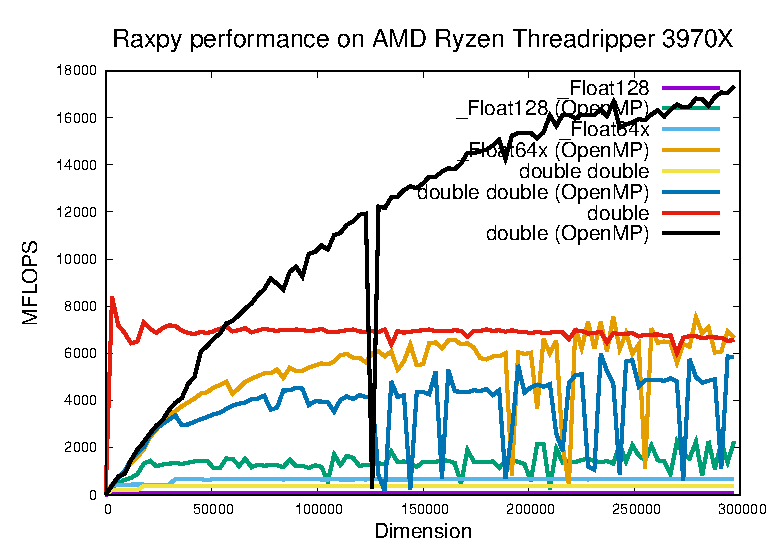
\includegraphics{Raxpy1.eps}
\end{center}
\vspace*{2.0cm}
\end{figure}


\begin{figure}
\caption{Raxpy performance on AMD Ryzen 3970X for {\tt quad-double}, {\tt GMP} and {\tt MPFR}, and (simple) OpenMP accelrated results. }
\label{raxpy2}
\begin{center}
\vspace*{-2.0cm}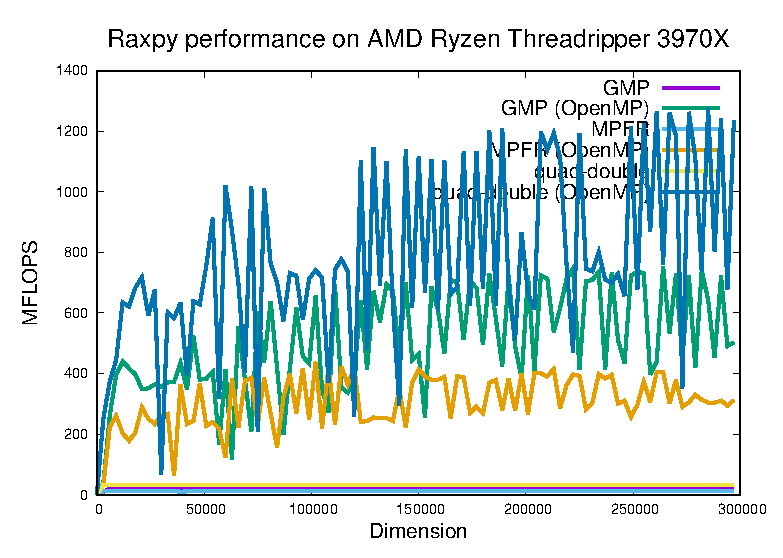
\includegraphics{Raxpy2.eps}
\end{center}
\vspace*{2.0cm}
\end{figure}

Users can take performance benchmark on your machine:
\begin{verbatim}
$ cd /home/docker/mplapack/benchmark/mpblas
$ bash -x go.Raxpy.sh
\end{verbatim}
and resultant files are {\tt Raxpy1.eps}  and {\tt Raxpy2.eps}. They correspond to Figure~\ref{raxpy1} and Figure~\ref{raxpy2}. 
\\
\\
In Figure~\ref{rgemm1}, we show the result of {\tt Rgemm} performance for {\tt \_Float128}, {\tt \_Float64x}, {\tt double} and  {\tt double-double}, and Figure~\ref{rgemm2} shows the {\tt Rgemm} performance for {\tt GMP}, {\tt MPFR}, and {\tt quad-double}, with and without optimization. We used CPU for AMD Ryzen 3970X, 256GB of DDR4 3200MHz memory (ECC is not enabled), and took benchmark inside Docker environment. GCC version was 9.3.0.

For these benchmarks, We performed {\tt Rgemm} calculations for each precision five times and took the average for OpenMP implementations and three times for the reference implementations. We used square matrices for the benchmarks.
The peak performance of the reference {\tt \_Float128} version was approximately 64 MFlops, and 2.4 GFlops for the OpenMP version. 

The peak performance of the reference {\tt \_Float64x} version
was approximately 665 MFlops, and 18.8 GFlops for the OpenMP version. The peak performance of the reference {\tt double-double} version was approximately 365 MFlops, and 11.2 GFlops for the OpenMP version. 
The double version is the fastest, and the peak was 6.8 GFlops for reference and 15 GFlops for the OpenMP version. These results are not competitive to OpenBLAS or Intel MKL. {\tt DGEMM} performance by OpenBLAS was 1.46 TBFlops with Ryzen Threadripper 3970X (This performance is almost 77\% of theoretical peak performance at rated core clock; 1.89 TFlops= 3.7[GHz] $\times$ 16 [AVX2] $\times$ 32 (cores)).

The peak performance of the reference {\tt GMP} version was 19 MFlops (512bit accuracy; default), and 693 MFlops OpenMP enabled.
The peak performance of the reference {\tt quad-double} version was 33 MFlops, and 1.3 GFlops OpenMP enabled.
The peak performance of reference {\tt MPFR} version was 11 MFlops (512bit accuracy; default), and 390 MFlops OpenMP enabled.
Thus, the {\tt MPFR} version is twice as slower than the {\tt GMP}.

In any case, enabling OpenMP will significantly increase the performance of {\tt Rgemm}. Moreover, the performances are stabler than {\tt Raxpy} results. 

\begin{figure}
\caption{Rgemm performance on AMD Ryzen 3970X for {\tt \_Float128}, {\tt \_Float64x}, {\tt double-double}, {\tt double} and (simple) OpenMP accelrated results. }
\label{rgemm1}
\begin{center}
\vspace*{-2.0cm}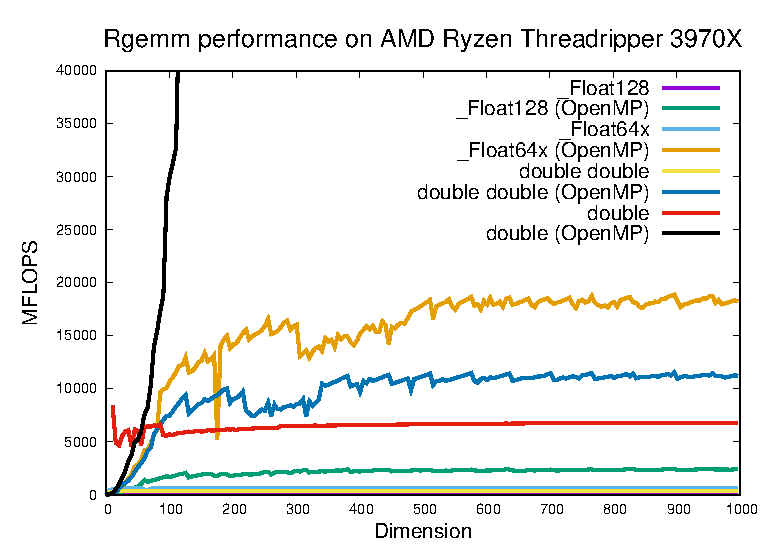
\includegraphics{Rgemm1.eps}
\end{center}
\end{figure}

\begin{figure}
\caption{Rgemm performance on AMD Ryzen 3970X for {\tt quad-double}, {\tt GMP} and {\tt MPFR}, and (simple) OpenMP accelrated results. }
\label{rgemm2}
\begin{center}
\vspace*{-2.0cm}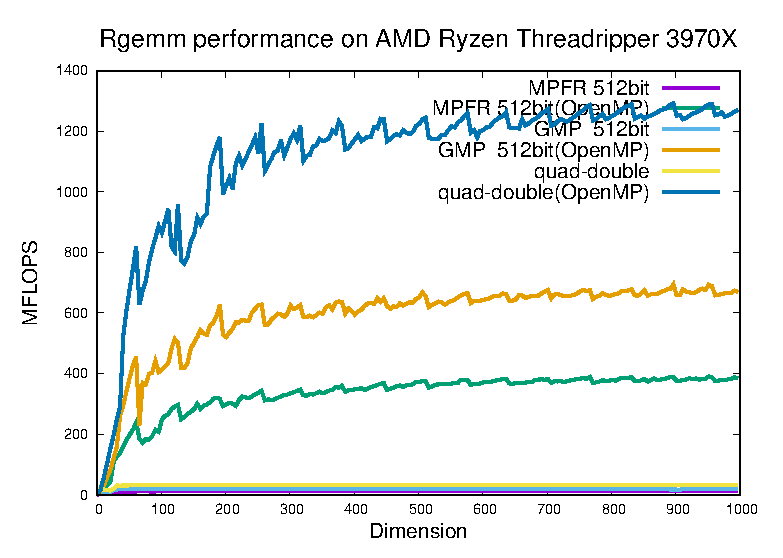
\includegraphics{Rgemm2.eps}
\end{center}
\vspace*{2.0cm}
\end{figure}

Users can take performance benchmark on your machine:
\begin{verbatim}
$ cd /home/docker/mplapack/benchmark/mpblas
$ bash -x go.Rgemm.sh
\end{verbatim}
and resultant files are {\tt Rgemm1.eps}  and {\tt Rgemm2.eps}. They correspond to Figure~\ref{rgemm1} and Figure~\ref{rgemm2}.

\section{History}
\label{sec:history}
M.N started developing MPLAPACK as a by-product of an arbitrary accurate semidefinite programming solver, SDPA-GMP, around 2006~\cite{JCP2008}. The first MPLAPACK (formerly MPACK) version, 0.0.1, was released in 2008-7-15. In 2009-2-5, we released SDPA-GMP 7.1.2, and MPLAPACK supports SDPA-GMP, SDPA-QD, and SDPA-DD~\cite{SDPA-GMP,sdpa-gmpgithub,sdpa-qdgithub,sdpa-ddgithub}. In 2010-01-13, we supported Windows via mingw32. In 2010-5-21, we supported MPFR. In 2012-10-13, we released a fast implementation of a double-double version of Rgemm for NVIDIA C2050~\cite{6424545,6495966}. In 2017-3-29, we moved the web site from \url{http://mplapack.sourceforge.net/} to \url{https://github.com/nakatamaho/mplapack/}. In 2021-4-1, we renamed our project to MPLAPACK. In 2021-4-11, we supported AArch64 and released 0.9.4. In 2021-10-1, we released 1.0.0.

\section{Related works}
\label{sec:relatedworks}
We can relate our work in two main directions. (i) acceleration of multiple-precision extension to BLAS (especially on GPU) and (ii) development of a multiple-precision version of linear algebra packages.

For (i), In 2009, Mukunoki\etal{}~\cite{HPC-137_1} implemented double-double version of matrix-matrix multiplication kernels for NVIDIA Tesla C1060 and evaluated the performance. In 2010, Mukunoki \etal{}~\cite{10.1007/978-3-642-28151-8_25} the quadruple precision Basic Linear Algebra Subprograms (BLAS) functions, AXPY, GEMV, and GEMM, on graphics processing units (GPUs), and evaluated their performance. On an NVIDIA Tesla C1060, their BLAS functions are approximately 30 times faster than the existing quadruple precision BLAS on an Intel Core i7 920.

In 2011, Nakasato~\cite{Nakasato2011AFG} implemented optimized dense matrix multiplication kernels for AMD Cypress GPU for various precisions. Their result includes double-double precision, and attained peak performance of 30 GFlops.

In 2012, Nakata~\etal{}~\cite{6495966} implemented double-double version of {\tt Rgemm} on NVIDIA C2050. In their implementation is complete {\tt Rgemm} implementation; thus, their implementation can be used for real applications; it can handle all the sizes in matrices, and supports transpose of each matrix. They attained 16.1GFlops with CPU-GPU transfer included, and 26.4GFlops (25.7GFlops with CPU-GPU transfer included. Moreover, they applied to semidefinite programming solver and attained ten times acceleration compared to CPU-only implementation.

In 2012, Yamada~\etal{} developed QPBLAS packages for CPUs~\cite{7965202}, as well as in the QPBLAS-GPU package for GPUs in 2013~\cite{qpblas-gpu}. These correspond to the complete set of double-double version parts of MPBLAS, accelerating CPU and GPUs. Note that memory alignment is different from MPBLAS and written in Fortran 90.

In 2014 and 2015, Kouya~\cite{Tomonori_Kouya2014,Tomonori_Kouya2016} implemented optimized  matrix-matrix multiplications using Strassen and Winograd algorithms using MPFR, double-double, and quad-double precisions and applied them to LU factorizations. Strassen and Winograd versions are twice as fast as double-double and quad-double precisions running one core using a simple blocking algorithm. Furthermore, there is no significant performance difference between the Strassen version and Winograd. However, when we used MPFR, the Winograd version was always faster. He also found a significant loss of accuracy when performing LU factorization using Strassen and Winograd versions. 

In 2016, Joldes \etal{} implemented CAMPARY: Cuda Multiple Precision Arithmetic Library and applied it to semi-definite programming~\cite{10.1007/978-3-319-42432-3_29}. However, it was a prototype implementation and somewhat slower than our CPU implementation of ours~\cite{SDPA-GMP}. In 2017, Joldes \etal{} implemented an improved version of CAMPARY~\cite{8023060}. The significant result of this paper is that they improved {\tt Rgemm} performance on GPU for various multiple-precision versions; 1.6GFlops for triple-double precision, 976MFlops for quadruple-precision, 660MFlops for quintuple-double, 453MFlops for sextuple-double, 200MFlops for octuple-double.

In 2019, Hishinuma \etal{} implimented {\tt Rgemm} kernels for double-double precision on MIMD type acclearlator PEZY-SC2~\cite{hishinuma2019pzqd}. 
The performance of their implementation of {\tt Rgemm} the PEZY-SC2 attained 75\% of the peak performance. This value is 20 times faster than an Intel Xeon E5-2618L v3, even including the communication time between the host CPU and the PEZY-SC2.

In 2020, Isopov \etal{}~\cite{ISUPOV2020105506} took a benchmark for several level-1 multi-precision routines for MPFR, ARPREC, MPDECIMAL, MPACK, GARPREC, CUMP,, and MPRES-BLAS. MPRES-BLAS is an ongoing effort to develop a multiple-precision version of BLAS like MPBLAS on GPUS~ The\cite{10.1007/978-3-030-64616-5_4}. MPRES-BLAS defines a new arbitrary precision type suited for GPUs and fastest among CAMPARY~\cite{10.1007/978-3-319-42432-3_29}, CUMP~\cite{Nakayama2011ImplementationOM} and GARPREC~\cite{Lu:2010:SEP:1869389.1869392} when the fractions range from 424bits to 848 bits.

In 2021, Kouya~\cite{10.1007/978-3-030-86976-2_14} acceralated {\tt dd\_real}, {\tt qd\_real} and triple-double precision version of {\tt Rgemm} with AVX2 using Strassen algorithm~\cite{STRASSEN1969}. 

For (ii), Kouya has long developed C libraries for multiple-precision calculation using GMP and MPFR, including matrix operations~\cite{BNCpack}. He calls them as BNCpack and MPIBNCPack. At least, we can back to 2003 to find there was MPIBNCpack version 0.1~\cite{MPIBNCPack01}. In 2011, version 0.7 had released, and it can solve linear equations and eigenvalue problems, and many multiple-precision functions not directly related to linear algebra. From version 0.8 (2013-03-11), BNCpack and MPIBNCpack are integrated~\cite{BNCpack,1710.01839}.

Saito developed ZKCM~\cite{SAITOH20132005}, a C++ library for multi-precision matrix computation for quantum computer simulation. He implemented matrix inversion, singular-value decomposition of a general matrix, the diagonalization of a Hermitian matrix, and other operations.

Arb is a C library for arbitrary-precision ball arithmetic developed by Johansson~\cite{1611.02831}. It uses ball arithmetic to track
numerical errors automatically.  It can perform and solve a wide range of matrix operations, e.g.,  LU factorization, inversion, eigenvalue problems, but it is not an extension of LAPACK to higher precision since employed arithmetic is different. 

Multiprecision Computing Toolbox by Advanpix for MATLAB is a toolbox of MATLAB, can solve many arbitrary precision matrix operations
like diagonalization of real and complex non-symmetric matrices, singular value decomposition with
outstanding performance. They seem to employ a similar approach to ours to convert LAPACK to multiple precision versions, but details are not open and do not replace LAPACK~\cite{advanpix}. Symbolic Math Toolbox (SMT) of Matlab also provides such functionalities~\cite{matlabsymbolic}.

RalphAS has been developing GenericSchur.jl~\cite{GenericSchur}, and it calculates Schur decomposition of matrices with generic floating-point element types in Julia. However, it is not a replacement for the LAPACK library.

Johansson~\etal{} also has been developing mpmath~\cite{mpmath} can handle linear algebra (linear system solving, LU factorization, matrix inverse, matrix norms, matrix exponentials/logarithms/square roots, eigenvalues, singular values, QR factorization), written in python, and it is not a replacement of LAPACK.

Mathematica~\cite{mathematica} has multiple-precision versions of the eigenvalue problem of non-symmetric matrices, singular value decomposition problems, and other solvers.

\section{Future plans}
\label{sec:futureplans}
In version 2.0.0, we finish RFP, complex version, and mixed-precision version, and in version 3.0.0, we plan to implement optimized MPFR C++ wrapper and drop GMP version.

\section*{Acknowledgement}

First, We are grateful to the LAPACK team for making an excellent library.
This work was supported by the Special Postdoctoral Researchers' Program of RIKEN (2008, 2009), Grant-in-Aid for Scientific Research (B) 21300017 from the Japan Society for the Promotion of Science (2009, 2010, 2011), Microsoft Research CORE6 (2010) and the Japan Society for the Promotion of Science (JSPS KAKENHI Grant no. 18H03206). 
The author would like to thank Dr. Imamura Toshiyuki. Dr. Nakasato Naohito, Dr. Fujisawa Katsuki, Dr. Kouya Tomonori, Dr. Takahashi Daisuke, Dr. Goto Kazushige, Dr. Himeno Ryutaro, Dr. Hishimuna Toshiaki, Dr. Katagiri Takahiro, Dr. Ogita Takeshi, Dr. Kashiwagi Masahide, Dr. Yuasa Fukuko, Dr. Ishikawa Tadashi, Dr. Geshi Masaaki and Mr. Minato Yuichiro for warm encouragement.

\bibliography{manual}

\end{document}